%%%%%%%%%%%%%%%%%%%%%%%%%%%%%%%%%%%%%%%%%%%%%%%%%%%%%%%%%%%%%%%
%% OXFORD THESIS TEMPLATE

% Use this template to produce a standard thesis that meets the Oxford University requirements for DPhil submission
%
% Originally by Keith A. Gillow (gillow@maths.ox.ac.uk), 1997
% Modified by Sam Evans (sam@samuelevansresearch.org), 2007
% Modified by John McManigle (john@oxfordechoes.com), 2015
% Modified by Ulrik Lyngs (ulrik.lyngs@cs.ox.ac.uk), 2018, for use with R Markdown
%
% Ulrik Lyngs, 25 Nov 2018: Following John McManigle, broad permissions are granted to use, modify, and distribute this software
% as specified in the MIT License included in this distribution's LICENSE file.
%
% John tried to comment this file extensively, so read through it to see how to use the various options.  Remember
% that in LaTeX, any line starting with a % is NOT executed.  Several places below, you have a choice of which line to use
% out of multiple options (eg draft vs final, for PDF vs for binding, etc.)  When you pick one, add a % to the beginning of
% the lines you don't want.


%%%%% CHOOSE PAGE LAYOUT
% The most common choices should be below.  You can also do other things, like replacing "a4paper" with "letterpaper", etc.

% This one will format for two-sided binding (ie left and right pages have mirror margins; blank pages inserted where needed):
%\documentclass[a4paper,twoside]{templates/ociamthesis}
% This one will format for one-sided binding (ie left margin > right margin; no extra blank pages):
%\documentclass[a4paper]{ociamthesis}
% This one will format for PDF output (ie equal margins, no extra blank pages):
%\documentclass[a4paper,nobind]{templates/ociamthesis}
%UL 2 Dec 2018: pass this in from YAML
\documentclass[a4paper, twoside]{templates/ociamthesis}


% UL 30 Nov 2018 pandoc puts lists in 'tightlist' command when no space between bullet points in Rmd file
\providecommand{\tightlist}{%
  \setlength{\itemsep}{0pt}\setlength{\parskip}{0pt}}
 
% UL 1 Dec 2018, fix to include code in shaded environments

%UL 2 Dec 2018 reduce whitespace around verbatim environments
\usepackage{etoolbox}
\makeatletter
\preto{\@verbatim}{\topsep=0pt \partopsep=0pt }
\makeatother

%UL 26 Mar 2019, enable strikethrough
\usepackage[normalem]{ulem}

%UL 15 Oct 2019, enable link highlighting to be turned off from YAML
\usepackage[colorlinks=false,pdfpagelabels,hidelinks=true]{hyperref}

%%%%% SELECT YOUR DRAFT OPTIONS
% Three options going on here; use in any combination.  But remember to turn the first two off before
% generating a PDF to send to the printer!

% This adds a "DRAFT" footer to every normal page.  (The first page of each chapter is not a "normal" page.)
\fancyfoot[C]{\emph{DRAFT Printed on \today}}

% This highlights (in blue) corrections marked with (for words) \mccorrect{blah} or (for whole
% paragraphs) \begin{mccorrection} . . . \end{mccorrection}.  This can be useful for sending a PDF of
% your corrected thesis to your examiners for review.  Turn it off, and the blue disappears.
\correctionstrue

%%%%% BIBLIOGRAPHY SETUP
% Note that your bibliography will require some tweaking depending on your department, preferred format, etc.
% The options included below are just very basic "sciencey" and "humanitiesey" options to get started.
% If you've not used LaTeX before, I recommend reading a little about biblatex/biber and getting started with it.
% If you're already a LaTeX pro and are used to natbib or something, modify as necessary.
% Either way, you'll have to choose and configure an appropriate bibliography format...

% The science-type option: numerical in-text citation with references in order of appearance.
% \usepackage[style=numeric-comp, sorting=none, backend=biber, doi=false, isbn=false]{biblatex}
% \newcommand*{\bibtitle}{References}

% The humanities-type option: author-year in-text citation with an alphabetical works cited.
% \usepackage[style=authoryear, sorting=nyt, backend=biber, maxcitenames=2, useprefix, doi=false, isbn=false]{biblatex}
% \newcommand*{\bibtitle}{Works Cited}

%UL 3 Dec 2018: set this from YAML in index.Rmd
\usepackage[style=authoryear, sorting=nyt, backend=biber, maxcitenames=2, useprefix, doi=false, isbn=false, uniquename=false]{biblatex}
\newcommand*{\bibtitle}{References}

% This makes the bibliography left-aligned (not 'justified') and slightly smaller font.
\renewcommand*{\bibfont}{\raggedright\small}

% Change this to the name of your .bib file (usually exported from a citation manager like Zotero or EndNote).
\addbibresource{references.bib}


% Uncomment this if you want equation numbers per section (2.3.12), instead of per chapter (2.18):
%\numberwithin{equation}{subsection}


%%%%% THESIS / TITLE PAGE INFORMATION
% Everybody needs to complete the following:
\title{Flexibility in avian\\
migration across scales}
\author{Benjamin Mark Van Doren}
\college{Somerville College}

% Master's candidates who require the alternate title page (with candidate number and word count)
% must also un-comment and complete the following three lines:
%\masterssubmissiontrue
%\candidateno{933516}
%\wordcount{28,815}

% Uncomment the following line if your degree also includes exams (eg most masters):
%\renewcommand{\submittedtext}{Submitted in partial completion of the}
% Your full degree name.  (But remember that DPhils aren't "in" anything.  They're just DPhils.)
\degree{Doctor of Philosophy}
% Term and year of submission, or date if your board requires (eg most masters)
\degreedate{Hilary 2020}


%%%%% YOUR OWN PERSONAL MACROS
% This is a good place to dump your own LaTeX macros as they come up.

% To make text superscripts shortcuts
	\renewcommand{\th}{\textsuperscript{th}} % ex: I won 4\th place
	\newcommand{\nd}{\textsuperscript{nd}}
	\renewcommand{\st}{\textsuperscript{st}}
	\newcommand{\rd}{\textsuperscript{rd}}

%%%%% THE ACTUAL DOCUMENT STARTS HERE
\begin{document}

%%%%% CHOOSE YOUR LINE SPACING HERE
% This is the official option.  Use it for your submission copy and library copy:
\setlength{\textbaselineskip}{22pt plus2pt}
% This is closer spacing (about 1.5-spaced) that you might prefer for your personal copies:
%\setlength{\textbaselineskip}{18pt plus2pt minus1pt}

% You can set the spacing here for the roman-numbered pages (acknowledgements, table of contents, etc.)
\setlength{\frontmatterbaselineskip}{17pt plus1pt minus1pt}

% UL: You can set the line and paragraph spacing here for the separate abstract page to be handed in to Examination schools
\setlength{\abstractseparatelineskip}{13pt plus1pt minus1pt}
\setlength{\abstractseparateparskip}{0pt plus 1pt}

% UL: You can set the general paragraph spacing here - I've set it to 2pt (was 0) so
% it's less claustrophobic
\setlength{\parskip}{2pt plus 1pt}


% Leave this line alone; it gets things started for the real document.
\setlength{\baselineskip}{\textbaselineskip}


%%%%% CHOOSE YOUR SECTION NUMBERING DEPTH HERE
% You have two choices.  First, how far down are sections numbered?  (Below that, they're named but
% don't get numbers.)  Second, what level of section appears in the table of contents?  These don't have
% to match: you can have numbered sections that don't show up in the ToC, or unnumbered sections that
% do.  Throughout, 0 = chapter; 1 = section; 2 = subsection; 3 = subsubsection, 4 = paragraph...

% The level that gets a number:
\setcounter{secnumdepth}{2}
% The level that shows up in the ToC:
\setcounter{tocdepth}{0}


%%%%% ABSTRACT SEPARATE
% This is used to create the separate, one-page abstract that you are required to hand into the Exam
% Schools.  You can comment it out to generate a PDF for printing or whatnot.
\begin{abstractseparate}
  This \emph{R Markdown} template is for writing an Oxford University thesis. The template is built using Yihui Xie's \texttt{bookdown} package, with heavy inspiration from Chester Ismay's \texttt{thesisdown} and the \texttt{OxThesis} \LaTeX~template (most recently adapted by John McManigle).
  
  This template's sample content include illustrations of how to write a thesis in R Markdown, and largely follows the structure from \href{https://ulyngs.github.io/rmarkdown-workshop-2019/}{this R Markdown workshop}.
  
  Congratulations for taking a step further into the lands of open, reproducible science by writing your thesis using a tool that allows you to transparently include tables and dynamically generated plots directly from the underlying data. Hip hooray!
\end{abstractseparate}

% JEM: Pages are roman numbered from here, though page numbers are invisible until ToC.  This is in
% keeping with most typesetting conventions.
\begin{romanpages}

% Title page is created here
\maketitle

%%%%% DEDICATION -- If you'd like one, un-comment the following.

%%%%% ACKNOWLEDGEMENTS -- Nothing to do here except comment out if you don't want it.
\begin{acknowledgements}
 	This is where you will normally thank your advisor, colleagues, family and friends, as well as funding and institutional support. In our case, we will give our praises to the people who developed the ideas and tools that allow us to push open science a little step forward by writing plain-text, transparent, and reproducible theses in R Markdown.

We must be grateful to John Gruber for inventing the original version of Markdown, to John MacFarlane for creating Pandoc (\url{http://pandoc.org}) which converts Markdown to a large number of output formats, and to Yihui Xie for creating \texttt{knitr} which introduced R Markdown as a way of embedding code in Markdown documents, and \texttt{bookdown} which added tools for technical and longer-form writing.

Special thanks to \href{http://chester.rbind.io}{Chester Ismay}, who created the \texttt{thesisdown} package that helped many a PhD student write their theses in R Markdown. And a very special tahnks to John McManigle, whose adaption of Sam Evans' adaptation of Keith Gillow's original maths template for writing an Oxford University DPhil thesis in \LaTeX~provided the template that I adapted for R Markdown.

Finally, profuse thanks to JJ Allaire, the founder and CEO of \href{http://rstudio.com}{RStudio}, and Hadley Wickham, the mastermind of the tidyverse without whom we'd all just given up and done data science in Python instead. Thanks for making data science easier, more accessible, and more fun for us all.

\begin{flushright}
Ulrik Lyngs \\
Linacre College, Oxford \\
2 December 2018
\end{flushright}
\end{acknowledgements}


%%%%% ABSTRACT -- Nothing to do here except comment out if you don't want it.
\begin{abstract}
	This \emph{R Markdown} template is for writing an Oxford University thesis. The template is built using Yihui Xie's \texttt{bookdown} package, with heavy inspiration from Chester Ismay's \texttt{thesisdown} and the \texttt{OxThesis} \LaTeX~template (most recently adapted by John McManigle).

This template's sample content include illustrations of how to write a thesis in R Markdown, and largely follows the structure from \href{https://ulyngs.github.io/rmarkdown-workshop-2019/}{this R Markdown workshop}.

Congratulations for taking a step further into the lands of open, reproducible science by writing your thesis using a tool that allows you to transparently include tables and dynamically generated plots directly from the underlying data. Hip hooray!
\end{abstract}

%%%%% MINI TABLES
% This lays the groundwork for per-chapter, mini tables of contents.  Comment the following line
% (and remove \minitoc from the chapter files) if you don't want this.  Un-comment either of the
% next two lines if you want a per-chapter list of figures or tables.

% This aligns the bottom of the text of each page.  It generally makes things look better.
\flushbottom

% This is where the whole-document ToC appears:
\tableofcontents


% Uncomment to generate a list of tables:
%%%%% LIST OF ABBREVIATIONS
% This example includes a list of abbreviations.  Look at text/abbreviations.tex to see how that file is
% formatted.  The template can handle any kind of list though, so this might be a good place for a
% glossary, etc.

% The Roman pages, like the Roman Empire, must come to its inevitable close.
\end{romanpages}

%%%%% CHAPTERS
% Add or remove any chapters you'd like here, by file name (excluding '.tex'):
\flushbottom

% all your chapters and appendices will appear here
\hypertarget{introduction}{%
\chapter*{Introduction}\label{introduction}}
\addcontentsline{toc}{chapter}{Introduction}

\adjustmtc

Welcome to the \emph{R Markdown} Oxford University thesis template.
This sample content is adapted from \href{https://github.com/ismayc/thesisdown}{\texttt{thesisdown}} and the formatting of PDF output is adapted from the \href{https://github.com/mcmanigle/OxThesis}{OxThesis LaTeX template}.
Hopefully, writing your thesis in R Markdown will provide a nicer interface to the OxThesis template if you haven't used TeX or LaTeX before.
More importantly, using \emph{R Markdown} allows you to embed chunks of code directly into your thesis and generate plots and tables directly from the underlying data, avoiding copy-paste steps.
This will get you into the habit of doing reproducible research, which benefits you long-term as a researcher, but also will greatly help anyone that is trying to reproduce or build upon your results down the road.

Using LaTeX together with \emph{Markdown} is more consistent than the output of a word processor, much less prone to corruption or crashing, and the resulting file is smaller than a Word file.
While you may never have had problems using Word in the past, your thesis is likely going to be about twice as large and complex as anything you've written before, taxing Word's capabilities.

\hypertarget{why-use-it}{%
\section*{Why use it?}\label{why-use-it}}
\addcontentsline{toc}{section}{Why use it?}

\emph{R Markdown} creates a simple and straightforward way to interface with the beauty of LaTeX.
Packages have been written in \textbf{R} to work directly with LaTeX to produce nicely formatting tables and paragraphs.
In addition to creating a user friendly interface to LaTeX, \emph{R Markdown} allows you to read in your data, analyze it and to visualize it using \textbf{R}, \textbf{Python} or other languages, and provide documentation and commentary on the results of your project.\\
Further, it allows for results of code output to be passed inline to the commentary of your results.
You'll see more on this later, focusing on \textbf{R}. If you are more into \textbf{Python} or something else, you can still use \emph{R Markdown} - see \href{https://bookdown.org/yihui/rmarkdown/language-engines.html}{`Other language engines'} in Yihui Xie's \href{https://bookdown.org/yihui/rmarkdown/language-engines.html}{\emph{R Markdown: The Definitive Guide}}.

\hypertarget{who-should-use-it}{%
\section*{Who should use it?}\label{who-should-use-it}}
\addcontentsline{toc}{section}{Who should use it?}

Anyone who needs to use data analysis, math, tables, a lot of figures, complex cross-references, or who just cares about reproducibility in research can benefit from using \emph{R Markdown}.
If you are working in `softer' fields, the user-friendly nature of the \emph{Markdown} syntax and its ability to keep track of and easily include figures, automatically generate a table of contents, index, references, table of figures, etc. should still make it of great benefit to your thesis project.

\hypertarget{programmed-and-flexible}{%
\chapter{Programmed and flexible: variation in migratory restlessness}\label{programmed-and-flexible}}

\minitoc 

\newpage

\begin{center}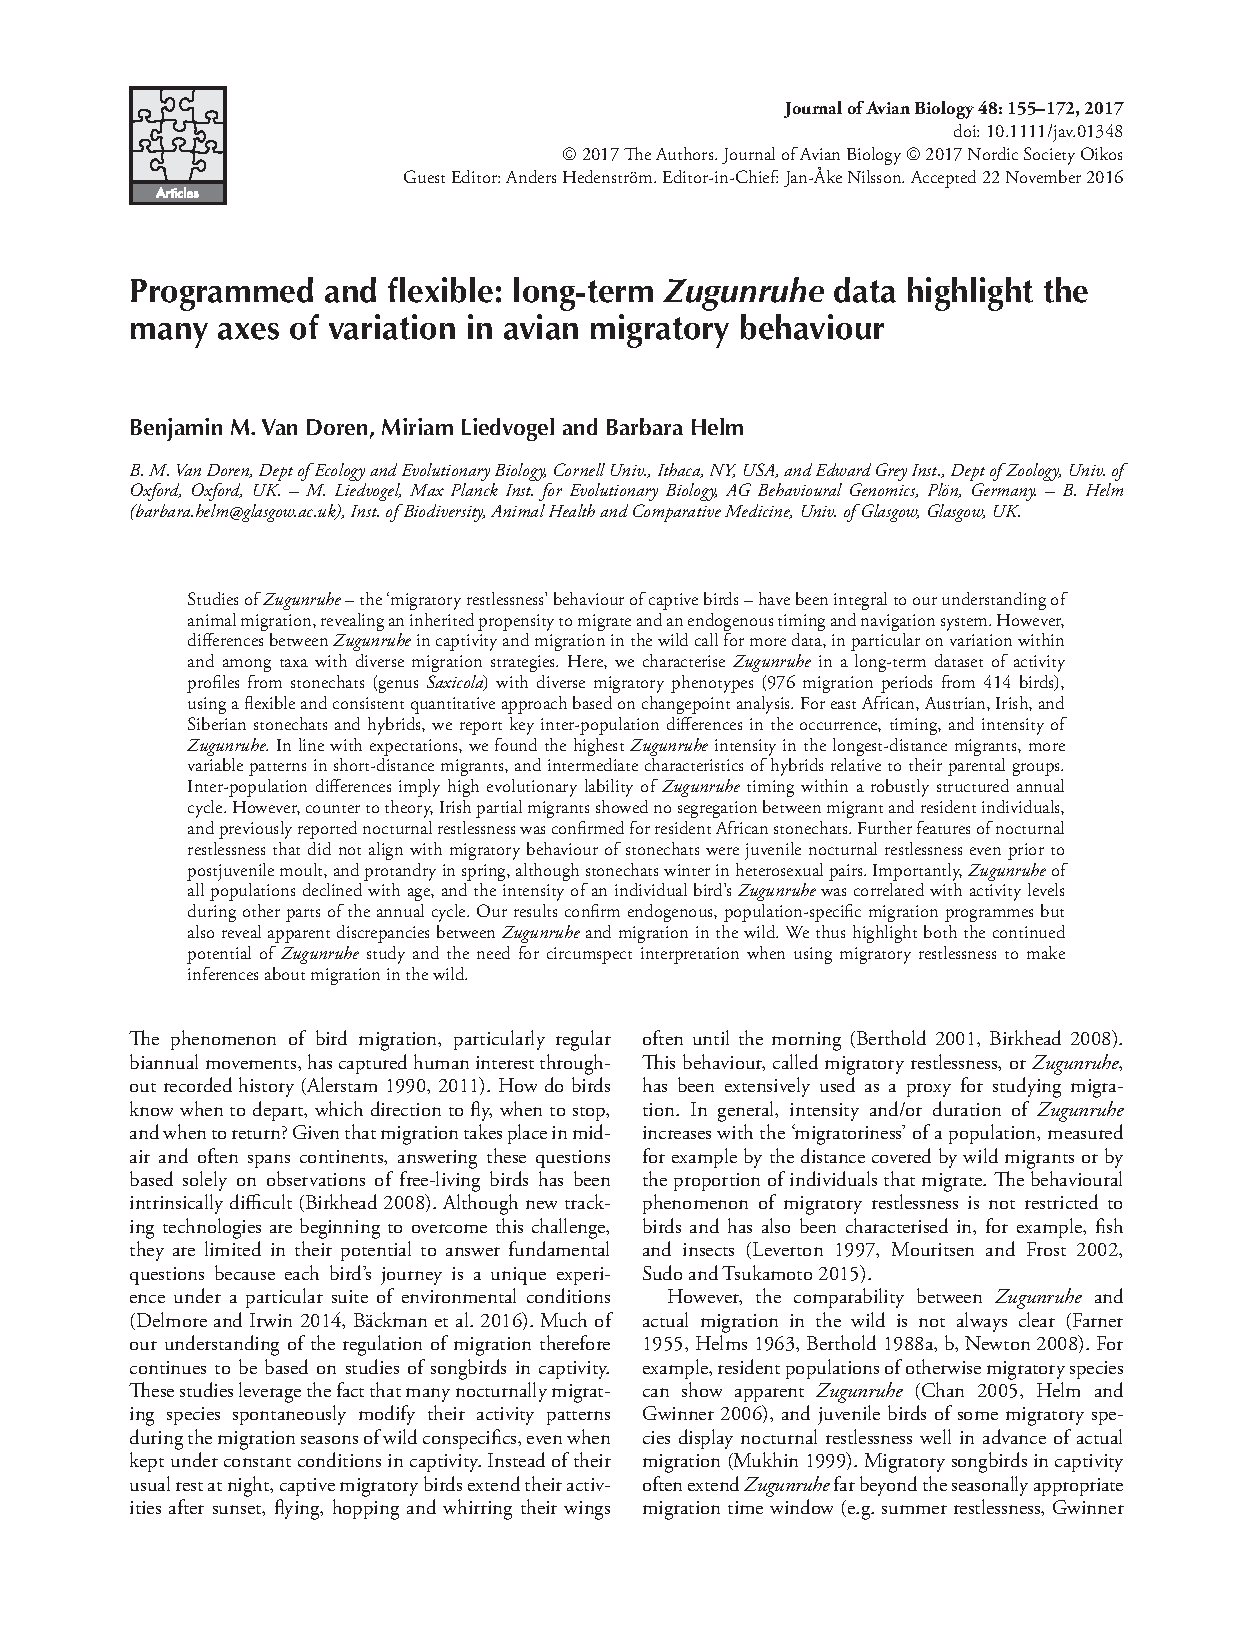
\includegraphics[width=1\linewidth]{pdf_chapters/zug/zug_crop_Part01} \end{center}

\begin{center}\includegraphics[width=1\linewidth]{pdf_chapters/zug/zug_crop_Part02} \end{center}

\begin{center}\includegraphics[width=1\linewidth]{pdf_chapters/zug/zug_crop_Part03} \end{center}

\begin{center}\includegraphics[width=1\linewidth]{pdf_chapters/zug/zug_crop_Part04} \end{center}

\begin{center}\includegraphics[width=1\linewidth]{pdf_chapters/zug/zug_crop_Part05} \end{center}

\begin{center}\includegraphics[width=1\linewidth]{pdf_chapters/zug/zug_crop_Part06} \end{center}

\begin{center}\includegraphics[width=1\linewidth]{pdf_chapters/zug/zug_crop_Part07} \end{center}

\begin{center}\includegraphics[width=1\linewidth]{pdf_chapters/zug/zug_crop_Part08} \end{center}

\begin{center}\includegraphics[width=1\linewidth]{pdf_chapters/zug/zug_crop_Part09} \end{center}

\begin{center}\includegraphics[width=1\linewidth]{pdf_chapters/zug/zug_crop_Part10} \end{center}

\begin{center}\includegraphics[width=1\linewidth]{pdf_chapters/zug/zug_crop_Part11} \end{center}

\begin{center}\includegraphics[width=1\linewidth]{pdf_chapters/zug/zug_crop_Part12} \end{center}

\begin{center}\includegraphics[width=1\linewidth]{pdf_chapters/zug/zug_crop_Part13} \end{center}

\begin{center}\includegraphics[width=1\linewidth]{pdf_chapters/zug/zug_crop_Part14} \end{center}

\begin{center}\includegraphics[width=1\linewidth]{pdf_chapters/zug/zug_crop_Part15} \end{center}

\begin{center}\includegraphics[width=1\linewidth]{pdf_chapters/zug/zug_crop_Part16} \end{center}

\begin{center}\includegraphics[width=1\linewidth]{pdf_chapters/zug/zug_crop_Part17} \end{center}

\begin{center}\includegraphics[width=1\linewidth]{pdf_chapters/zug/zug_crop_Part18} \end{center}

\begin{verbatim}
## \pagebreak
\end{verbatim}

\includegraphics[width=1\linewidth]{pdf_chapters/zug/zug_supp_crop_Part01}
\includegraphics[width=1\linewidth]{pdf_chapters/zug/zug_supp_crop_Part02}
\includegraphics[width=1\linewidth]{pdf_chapters/zug/zug_supp_crop_Part03}
\includegraphics[width=1\linewidth]{pdf_chapters/zug/zug_supp_crop_Part04}
\includegraphics[width=1\linewidth]{pdf_chapters/zug/zug_supp_crop_Part05}
\includegraphics[width=1\linewidth]{pdf_chapters/zug/zug_supp_crop_Part06}
\includegraphics[width=1\linewidth]{pdf_chapters/zug/zug_supp_crop_Part07}
\includegraphics[width=1\linewidth]{pdf_chapters/zug/zug_supp_crop_Part08}
\includegraphics[width=1\linewidth]{pdf_chapters/zug/zug_supp_crop_Part09}
\includegraphics[width=1\linewidth]{pdf_chapters/zug/zug_supp_crop_Part10}
\includegraphics[width=1\linewidth]{pdf_chapters/zug/zug_supp_crop_Part11}
\includegraphics[width=1\linewidth]{pdf_chapters/zug/zug_supp_crop_Part12}
\includegraphics[width=1\linewidth]{pdf_chapters/zug/zug_supp_crop_Part13}
\includegraphics[width=1\linewidth]{pdf_chapters/zug/zug_supp_crop_Part14}
\includegraphics[width=1\linewidth]{pdf_chapters/zug/zug_supp_crop_Part15}
\includegraphics[width=1\linewidth]{pdf_chapters/zug/zug_supp_crop_Part16}
\includegraphics[width=1\linewidth]{pdf_chapters/zug/zug_supp_crop_Part17}
\includegraphics[width=1\linewidth]{pdf_chapters/zug/zug_supp_crop_Part18}
\includegraphics[width=1\linewidth]{pdf_chapters/zug/zug_supp_crop_Part19}



\begin{savequote}
Neque porro quisquam est qui dolorem ipsum quia dolor sit amet,
consectetur, adipisci velit\ldots{}

There is no one who loves pain itself, who seeks after it and wants to
have it, simply because it is pain\ldots{}
\qauthor{--- Cicero's \emph{de Finibus Bonorum et Malorum}.}\end{savequote}

\hypertarget{evolutionary-response}{%
\chapter{Evolutionary response to climate change in migratory pied flycatchers}\label{evolutionary-response}}

\minitoc 

\newpage

\begin{center}\includegraphics[width=1\linewidth]{pdf_chapters/pied/pied_crop_Part01} \end{center}

\begin{center}\includegraphics[width=1\linewidth]{pdf_chapters/pied/pied_crop_Part02} \end{center}

\begin{center}\includegraphics[width=1\linewidth]{pdf_chapters/pied/pied_crop_Part03} \end{center}

\begin{center}\includegraphics[width=1\linewidth]{pdf_chapters/pied/pied_crop_Part04} \end{center}

\begin{center}\includegraphics[width=1\linewidth]{pdf_chapters/pied/pied_crop_Part05} \end{center}

\begin{center}\includegraphics[width=1\linewidth]{pdf_chapters/pied/pied_crop_Part06} \end{center}

\begin{center}\includegraphics[width=1\linewidth]{pdf_chapters/pied/pied_crop_Part07} \end{center}

\begin{center}\includegraphics[width=1\linewidth]{pdf_chapters/pied/pied_crop_Part08} \end{center}

\begin{center}\includegraphics[width=1\linewidth]{pdf_chapters/pied/pied_crop_Part09} \end{center}

\begin{center}\includegraphics[width=1\linewidth]{pdf_chapters/pied/pied_crop_Part10} \end{center}

\begin{verbatim}
## \pagebreak
\end{verbatim}

\includegraphics[width=1\linewidth]{pdf_chapters/pied/pied_supp_crop_Part1}
\includegraphics[width=1\linewidth]{pdf_chapters/pied/pied_supp_crop_Part2}
\includegraphics[width=1\linewidth]{pdf_chapters/pied/pied_supp_crop_Part3}
\includegraphics[width=1\linewidth]{pdf_chapters/pied/pied_supp_crop_Part4}
\includegraphics[width=1\linewidth]{pdf_chapters/pied/pied_supp_crop_Part5}
\includegraphics[width=1\linewidth]{pdf_chapters/pied/pied_supp_crop_Part6}
\includegraphics[width=1\linewidth]{pdf_chapters/pied/pied_supp_crop_Part7}

--- Cicero's \emph{de Finibus Bonorum et Malorum}. --- Cicero's \emph{de Finibus Bonorum et Malorum}.

\begin{savequote}
Neque porro quisquam est qui dolorem ipsum quia dolor sit amet,
consectetur, adipisci velit\ldots{}

There is no one who loves pain itself, who seeks after it and wants to
have it, simply because it is pain\ldots{}
\qauthor{--- Cicero's \emph{de Finibus Bonorum et Malorum}.}\end{savequote}

\hypertarget{continental-system}{%
\chapter{A continental system for forecasting bird migration}\label{continental-system}}

\minitoc 

\newpage

\begin{center}\includegraphics[width=1\linewidth]{pdf_chapters/forecast/forecast_crop_Part1} \end{center}

\begin{center}\includegraphics[width=1\linewidth]{pdf_chapters/forecast/forecast_crop_Part2} \end{center}

\begin{center}\includegraphics[width=1\linewidth]{pdf_chapters/forecast/forecast_crop_Part3} \end{center}

\begin{verbatim}
## \pagebreak
\end{verbatim}

\includegraphics[width=1\linewidth]{pdf_chapters/forecast/forecast_supp_crop_Part01}
\includegraphics[width=1\linewidth]{pdf_chapters/forecast/forecast_supp_crop_Part02}
\includegraphics[width=1\linewidth]{pdf_chapters/forecast/forecast_supp_crop_Part03}
\includegraphics[width=1\linewidth]{pdf_chapters/forecast/forecast_supp_crop_Part04}
\includegraphics[width=1\linewidth]{pdf_chapters/forecast/forecast_supp_crop_Part05}
\includegraphics[width=1\linewidth]{pdf_chapters/forecast/forecast_supp_crop_Part06}
\includegraphics[width=1\linewidth]{pdf_chapters/forecast/forecast_supp_crop_Part07}
\includegraphics[width=1\linewidth]{pdf_chapters/forecast/forecast_supp_crop_Part08}
\includegraphics[width=1\linewidth]{pdf_chapters/forecast/forecast_supp_crop_Part09}
\includegraphics[width=1\linewidth]{pdf_chapters/forecast/forecast_supp_crop_Part10}
\includegraphics[width=1\linewidth]{pdf_chapters/forecast/forecast_supp_crop_Part11}
\includegraphics[width=1\linewidth]{pdf_chapters/forecast/forecast_supp_crop_Part12}
\includegraphics[width=1\linewidth]{pdf_chapters/forecast/forecast_supp_crop_Part13}
\includegraphics[width=1\linewidth]{pdf_chapters/forecast/forecast_supp_crop_Part14}
\includegraphics[width=1\linewidth]{pdf_chapters/forecast/forecast_supp_crop_Part15}
\includegraphics[width=1\linewidth]{pdf_chapters/forecast/forecast_supp_crop_Part16}
\includegraphics[width=1\linewidth]{pdf_chapters/forecast/forecast_supp_crop_Part17}
\includegraphics[width=1\linewidth]{pdf_chapters/forecast/forecast_supp_crop_Part18}

--- Cicero's \emph{de Finibus Bonorum et Malorum}. --- Cicero's \emph{de Finibus Bonorum et Malorum}.

\begin{savequote}
Neque porro quisquam est qui dolorem ipsum quia dolor sit amet,
consectetur, adipisci velit\ldots{}

There is no one who loves pain itself, who seeks after it and wants to
have it, simply because it is pain\ldots{}
\qauthor{--- Cicero's \emph{de Finibus Bonorum et Malorum}.}\end{savequote}

\hypertarget{high-intensity-lights}{%
\chapter{High-intensity urban light installation dramatically alters bird migration}\label{high-intensity-lights}}

\minitoc 

\newpage

\begin{center}\includegraphics[width=1\linewidth]{pdf_chapters/lights/lights_crop_Part1} \end{center}

\begin{center}\includegraphics[width=1\linewidth]{pdf_chapters/lights/lights_crop_Part2} \end{center}

\begin{center}\includegraphics[width=1\linewidth]{pdf_chapters/lights/lights_crop_Part3} \end{center}

\begin{center}\includegraphics[width=1\linewidth]{pdf_chapters/lights/lights_crop_Part4} \end{center}

\begin{center}\includegraphics[width=1\linewidth]{pdf_chapters/lights/lights_crop_Part5} \end{center}

\begin{center}\includegraphics[width=1\linewidth]{pdf_chapters/lights/lights_crop_Part6} \end{center}

\begin{verbatim}
## \pagebreak
\end{verbatim}

\includegraphics[width=1\linewidth]{pdf_chapters/lights/lights_supp_crop_Part01}
\includegraphics[width=1\linewidth]{pdf_chapters/lights/lights_supp_crop_Part02}
\includegraphics[width=1\linewidth]{pdf_chapters/lights/lights_supp_crop_Part03}
\includegraphics[width=1\linewidth]{pdf_chapters/lights/lights_supp_crop_Part04}
\includegraphics[width=1\linewidth]{pdf_chapters/lights/lights_supp_crop_Part05}
\includegraphics[width=1\linewidth]{pdf_chapters/lights/lights_supp_crop_Part06}
\includegraphics[width=1\linewidth]{pdf_chapters/lights/lights_supp_crop_Part07}
\includegraphics[width=1\linewidth]{pdf_chapters/lights/lights_supp_crop_Part08}
\includegraphics[width=1\linewidth]{pdf_chapters/lights/lights_supp_crop_Part09}
\includegraphics[width=1\linewidth]{pdf_chapters/lights/lights_supp_crop_Part10}
\includegraphics[width=1\linewidth]{pdf_chapters/lights/lights_supp_crop_Part11}
\includegraphics[width=1\linewidth]{pdf_chapters/lights/lights_supp_crop_Part12}
\includegraphics[width=1\linewidth]{pdf_chapters/lights/lights_supp_crop_Part13}
\includegraphics[width=1\linewidth]{pdf_chapters/lights/lights_supp_crop_Part14}
\includegraphics[width=1\linewidth]{pdf_chapters/lights/lights_supp_crop_Part15}
\includegraphics[width=1\linewidth]{pdf_chapters/lights/lights_supp_crop_Part16}
\includegraphics[width=1\linewidth]{pdf_chapters/lights/lights_supp_crop_Part17}
\includegraphics[width=1\linewidth]{pdf_chapters/lights/lights_supp_crop_Part18}
\includegraphics[width=1\linewidth]{pdf_chapters/lights/lights_supp_crop_Part19}
\includegraphics[width=1\linewidth]{pdf_chapters/lights/lights_supp_crop_Part20}
\includegraphics[width=1\linewidth]{pdf_chapters/lights/lights_supp_crop_Part21}
\includegraphics[width=1\linewidth]{pdf_chapters/lights/lights_supp_crop_Part22}
\includegraphics[width=1\linewidth]{pdf_chapters/lights/lights_supp_crop_Part23}
\includegraphics[width=1\linewidth]{pdf_chapters/lights/lights_supp_crop_Part24}
\includegraphics[width=1\linewidth]{pdf_chapters/lights/lights_supp_crop_Part25}
\includegraphics[width=1\linewidth]{pdf_chapters/lights/lights_supp_crop_Part26}
\includegraphics[width=1\linewidth]{pdf_chapters/lights/lights_supp_crop_Part27}
\includegraphics[width=1\linewidth]{pdf_chapters/lights/lights_supp_crop_Part28}
\includegraphics[width=1\linewidth]{pdf_chapters/lights/lights_supp_crop_Part29}
\includegraphics[width=1\linewidth]{pdf_chapters/lights/lights_supp_crop_Part30}
\includegraphics[width=1\linewidth]{pdf_chapters/lights/lights_supp_crop_Part31}
\includegraphics[width=1\linewidth]{pdf_chapters/lights/lights_supp_crop_Part32}
\includegraphics[width=1\linewidth]{pdf_chapters/lights/lights_supp_crop_Part33}
\includegraphics[width=1\linewidth]{pdf_chapters/lights/lights_supp_crop_Part34}
\includegraphics[width=1\linewidth]{pdf_chapters/lights/lights_supp_crop_Part35}
\includegraphics[width=1\linewidth]{pdf_chapters/lights/lights_supp_crop_Part36}
\includegraphics[width=1\linewidth]{pdf_chapters/lights/lights_supp_crop_Part37}
\includegraphics[width=1\linewidth]{pdf_chapters/lights/lights_supp_crop_Part38}
\includegraphics[width=1\linewidth]{pdf_chapters/lights/lights_supp_crop_Part39}
\includegraphics[width=1\linewidth]{pdf_chapters/lights/lights_supp_crop_Part40}
\includegraphics[width=1\linewidth]{pdf_chapters/lights/lights_supp_crop_Part41}
\includegraphics[width=1\linewidth]{pdf_chapters/lights/lights_supp_crop_Part42}
\includegraphics[width=1\linewidth]{pdf_chapters/lights/lights_supp_crop_Part43}
\includegraphics[width=1\linewidth]{pdf_chapters/lights/lights_supp_crop_Part44}
\includegraphics[width=1\linewidth]{pdf_chapters/lights/lights_supp_crop_Part45}
\includegraphics[width=1\linewidth]{pdf_chapters/lights/lights_supp_crop_Part46}
\includegraphics[width=1\linewidth]{pdf_chapters/lights/lights_supp_crop_Part47}
\includegraphics[width=1\linewidth]{pdf_chapters/lights/lights_supp_crop_Part48}
\includegraphics[width=1\linewidth]{pdf_chapters/lights/lights_supp_crop_Part49}
\includegraphics[width=1\linewidth]{pdf_chapters/lights/lights_supp_crop_Part50}
\includegraphics[width=1\linewidth]{pdf_chapters/lights/lights_supp_crop_Part51}
\includegraphics[width=1\linewidth]{pdf_chapters/lights/lights_supp_crop_Part52}
\includegraphics[width=1\linewidth]{pdf_chapters/lights/lights_supp_crop_Part53}
\includegraphics[width=1\linewidth]{pdf_chapters/lights/lights_supp_crop_Part54}
\includegraphics[width=1\linewidth]{pdf_chapters/lights/lights_supp_crop_Part55}
\includegraphics[width=1\linewidth]{pdf_chapters/lights/lights_supp_crop_Part56}
\includegraphics[width=1\linewidth]{pdf_chapters/lights/lights_supp_crop_Part57}
\includegraphics[width=1\linewidth]{pdf_chapters/lights/lights_supp_crop_Part58}
\includegraphics[width=1\linewidth]{pdf_chapters/lights/lights_supp_crop_Part59}
\includegraphics[width=1\linewidth]{pdf_chapters/lights/lights_supp_crop_Part60}
\includegraphics[width=1\linewidth]{pdf_chapters/lights/lights_supp_crop_Part61}
\includegraphics[width=1\linewidth]{pdf_chapters/lights/lights_supp_crop_Part62}
\includegraphics[width=1\linewidth]{pdf_chapters/lights/lights_supp_crop_Part63}
\includegraphics[width=1\linewidth]{pdf_chapters/lights/lights_supp_crop_Part64}

--- Cicero's \emph{de Finibus Bonorum et Malorum}. --- Cicero's \emph{de Finibus Bonorum et Malorum}.

\begin{savequote}
Neque porro quisquam est qui dolorem ipsum quia dolor sit amet,
consectetur, adipisci velit\ldots{}

There is no one who loves pain itself, who seeks after it and wants to
have it, simply because it is pain\ldots{}
\qauthor{--- Cicero's \emph{de Finibus Bonorum et Malorum}.}\end{savequote}

\hypertarget{blackcap-geo}{%
\chapter{Versatile migratory strategies in blackcaps}\label{blackcap-geo}}

\minitoc 

\hypertarget{summary}{%
\section{Summary}\label{summary}}

Migration is ubiquitous in the animal kingdom and may play a key role in promoting reproductive isolation \autocite{bearhopAssortativeMatingMechanism2005,benschMorphologicalMolecularVariation1999,helbigSESWmigratingBlackcap1991,irwinSiberianMigratoryDivides2005} and underpinning responses to environmental change \autocite{bertholdRapidMicroevolutionMigratory1992,plummerSupplementaryFeedingGardens2015}.
Migratory divides are contact zones between populations with different migratory phenotypes and ideal natural laboratories for studying the evolution of migration \autocite{delmoreGeneticsSeasonalMigration2016,delmoreHybridSongbirdsEmploy2014}.
The Eurasian blackcap (\emph{Sylvia atricapilla}) is a songbird that exhibits a migratory divide in Central Europe between populations that migrate southwest (SW) and southeast (SE) in autumn \autocite{helbigInheritanceMigratoryDirection1991,helbigPopulationDifferentiationMigratory1992,helbigSESWmigratingBlackcap1991} and has recently established a wintering population in Britain \autocite{bearhopAssortativeMatingMechanism2005,bertholdMigratoryBehaviourPopulation1988,bertholdRapidMicroevolutionMigratory1992,leachWinteringBlackcapsBritain1981}. We tracked 106 annual migrations of 98 blackcaps captured across their range to characterize both the migratory divide and novel wintering strategy.
Blackcaps to the west and east of the divide used predominantly SW and SE directions, respectively, but close to the contact zone many individuals took intermediate (S) routes. At 14.0ºE, we documented a sharp transition (22 km) in migratory direction from SW to SE, implying a strong selection gradient across the divide.
Blackcaps wintering in Britain took northwesterly migration routes from continental European breeding grounds. They originated from a surprisingly extensive area, spanning 2000 km of the breeding range. British winterers bred in sympatry with SW-bound migrants but arrived 10 days earlier on the breeding grounds, suggesting some potential for assortative mating by timing.
Overall, our data reveal complex variation in songbird migration and suggest that selection can maintain variation in migration direction across short distances while enabling the spread of a novel strategy across a wide range.

Keywords: migration, divide, timing, songbird, speciation, assortative mating

\hypertarget{results-and-discussion}{%
\section{Results and Discussion}\label{results-and-discussion}}

Pioneering studies of blackcaps revealed that songbird migration has a genetic basis and can rapidly evolve, and these findings underlie much of our current understanding of bird migration \autocite{bearhopAssortativeMatingMechanism2005,bertholdEvolutionaryAspectsMigratory1988,bertholdHeritabilityMigratoryActivity1994,bertholdRapidMicroevolutionMigratory1992,helbigGeneticBasisMode1996,helbigInheritanceMigratoryDirection1991,muellerIdentificationGeneAssociated2011,pulidoCurrentSelectionLower2010,pulidoFrequencyMigrantsMigratory1996,pulidoGeneticsEvolutionAvian2007,pulidoHeritabilityTimingAutumn2001,rolshausenContemporaryEvolutionReproductive2009}.
Today, blackcaps may offer important insight into adaptation to environmental change, as recent population increases \autocite{ebcc/birdlife/rspb/csoTrendsCommonBirds2018} and new routes \autocite{bertholdRapidMicroevolutionMigratory1992} illustrate how this species has successfully kept pace with a changing world.
A major limitation of past studies on blackcaps has been a reliance on indirect experiments in captivity (see \autocite{vandorenProgrammedFlexibleLongterm2017,zunigaAbruptSwitchMigratory2016}) and infrequent recaptures of ringed birds to infer phenotypes.
We sought to bridge this gap by intensively tracking blackcaps in the wild across the species' range, examining the processes shaping migratory divides and contemporary migratory change, and placing our results in an evolutionary context.

\hypertarget{tracking-blackcaps-across-a-migratory-divide}{%
\subsection{Tracking blackcaps across a migratory divide}\label{tracking-blackcaps-across-a-migratory-divide}}

Ringing and orientation studies suggest that a migratory divide exists in Central Europe between blackcaps that migrate SW and SE, running north-south at 14ºE \autocite{helbigPopulationDifferentiationMigratory1992,helbigSESWmigratingBlackcap1991}. We tracked 41 annual migrations of 36 adult male blackcaps from breeding territories across the divide in Austria. To contrast behavioral variation inside and outside the divide, we also tracked blackcaps (3 F, 39 M) from breeding sites in the Netherlands (N=21), west Austria (N=6), central Germany (N=4), northern Poland (N=8), and east Austria (N=3). We expected to find a mix of strategies in the divide versus pure SW and SE directions at sites west and east of the divide, respectively.

Our tracks from the divide area clearly demonstrate the existence of a migratory divide (Figures \ref{fig:geo-plot-4} and \ref{fig:bearings-map-austria}, Figure \ref{fig:divide-routes-fig}). We estimated each blackcap's autumn migration direction by drawing a rhumb line between breeding and wintering areas. Migration directions varied between 130 and 288º. Intermediate (S) routes were more common (53.7\%) than SE (26.8\%) and SW (17.1\%) strategies (Figure \ref{fig:geo-plot-4}A). One individual from within the divide migrated NW to winter in Britain. Multi-year tracks revealed highly repeatable routes (Figure \ref{fig:repeat-fig}). Among-individual variation in migratory direction was considerably greater in the divide (Figure \ref{fig:var-fig-edit}), suggesting that the contact between migratory phenotypes gives rise to increased diversity of behaviors.

A cline analysis using migration directions suggests that strong selection is maintaining the divide. Specifically, we examined the change in directions from western Austria (entirely SW), through the divide to eastern Austria (largely SE) (Figure \ref{fig:bearings-map-austria}; see Methods). We fit a cline through these directions to characterize its center and width. Clines maintained by selection should be narrow relative to dispersal distance, with a rapid transition between phenotypes \autocite{bartonGeneticAnalysisHybrid1993}. Our data showed this pattern: the center of the cline occurred at 14.0ºE {[}interval within two log-likelihood units: 13.8--14.2º{]} and its width was only 22 km {[}2LL: 14--93 km{]}. This transition from SW to SE directions is very narrow compared to average natal dispersal distance in blackcaps (41.2 km \autocite{paradisPatternsNatalBreeding1998}).

Our data do not allow direct identification of the source of selection, but possible processes include prezygotic selection for assortative mating and postzygotic selection reducing the fitness of hybrids. We discuss the potential for assortative mating in the next section. Helbig \autocite{helbigInheritanceMigratoryDirection1991} selectively mated SW and SE blackcaps in captivity and observed intermediate orientations in their offspring. He argued that these hybrids would experience lower fitness through reduced survival, as they would have to cross the Alps, Mediterranean Sea, and Sahara Desert. This is a widely held hypothesis today \autocite{benschGeneticMorphologicalFeather2009,helbigInheritanceMigratoryDirection1991,irwinSiberianMigratoryDivides2005}, but our data do not necessarily support it, as a considerable number of the birds we tracked successfully took intermediate routes, survived, and returned to be recaptured. Most of these birds encountered portions of the Alps, but many did not cross the Mediterranean, in which case they never encountered this barrier or the Sahara Desert. Many of the birds that wintered in Africa navigated around the Mediterranean, and others used Italy as a land bridge (Figure \ref{fig:geo-plot-4} and \ref{fig:divide-routes-fig}).

There is one important caveat: to maximize recapture success, we exclusively tracked adult birds, which had already completed at least one migration. It is possible that some blackcaps attempt to migrate over the Mediterranean and Sahara but do not survive to adulthood. Indeed, there is a striking deficit of birds wintering in Africa around 5ºE and 15ºE (Figure \ref{fig:geo-plot-4} and \ref{fig:divide-routes-fig}; note that birds from Dutch and Polish populations did winter in these areas). This deficit would not have been present in Helbig's work because he was not tracking free-flying birds. Alvarado et al.~\autocite{alvaradoIntegrativeTrackingMethods2014} argued similarly after failing to recover hybrids in a divide between hermit thrushes (\emph{Catharus guttatus}). At present, tracking of small songbirds is limited to archival tags not capable of transmitted daily location estimates, so we cannot address this idea further.



\begin{figure}
\includegraphics[width=1\linewidth]{_main_files/figure-latex/geo-plot-4-1} \caption{\textbf{Wintering (i.e.~non-breeding) and breeding locations of migratory blackcaps.} Wintering and breeding location estimates made with \texttt{GeoLight} shown with closed and open circles, respectively. Uncertainty in latitude estimation is indicated with vertical bars, which show estimates for sun angles higher and lower than the calibrated sun angle by 1º (following \autocite{hiemerFirstTracksIndividual2018}). Colors indicate SW (orange)/intermediate (green)/SE (blue)/Britain (black) phenotypes, categorized by wintering location. \textbf{(A)} Winter sites of blackcaps breeding within the central European migratory divide transect in Austria. \textbf{(B)} Winter sites of blackcaps breeding in Austria east or west of the migratory divide. \textbf{(C)} Winter sites of blackcaps breeding in the Netherlands, southern Germany, and northern Poland. \textbf{(D)} Breeding sites of blackcaps wintering in Britain.}\label{fig:geo-plot-4}
\end{figure}



\begin{figure}
\includegraphics[width=1\linewidth]{_main_files/figure-latex/bearings-map-austria-1} \caption{\textbf{Autumn migration directions of blackcaps in Central Europe.} \textbf{(A)} Gray lines indicate migration directions of individual blackcaps, and blue lines indicate the mean direction at each capture site. In both panels, the solid vertical red line indicates the estimated cline center, and the red shading shows estimated cline width. \textbf{(B)} Autumn migration direction by breeding longitude for Austrian blackcaps, with the maximum likelihood cline plotted. Small gray dots show the directions of individual blackcaps, and large black dots represent groupings of birds treated as sites for the analysis with \texttt{hzar}, which requires site-based input data. The dotted horizontal line is 180º (due south).}\label{fig:bearings-map-austria}
\end{figure}



\begin{figure}
\includegraphics[width=1\linewidth]{/Users/Benjamin/Documents/Oxford/Blackcaps/Blackcap_Geolocator_Analysis/blackcap_geo_comparative/flightr/figures_compiled/fl_all_4Feb2020_thresh1max10_b1500_nomask/draft_figures/variation_edit-01} \caption{\textbf{Variation in autumn migration direction by breeding area.} \textbf{(A)} Migration direction of tracked blackcaps caught at breeding sites across continental Europe. Each line points in the direction of autumn migration and is colored by winter region (SW=orange, intermediate=green, SE=blue, and NW (Britain)=black). Levene's test among sites with 5 or more tracked birds showed significantly higher variation in the area of the migratory divide: divide vs.~Netherlands F\textsubscript{1,61}=29.3, P\textless0.0001; divide vs.~west Austria F\textsubscript{1,45}=6.36, P=0.015; divide vs.~Poland F\textsubscript{1,47}=7.68, P=0.008 (excluding the NW migrant does not appreciably change this result). \textbf{(B)} Each dot shows the migration direction of one tracked blackcap (colored as in A). \textbf{(C)} Circular variance of autumn migration directions at each capture site, categorized by breeding region. Dot size shows the sample size at each site.}\label{fig:var-fig-edit}
\end{figure}

\hypertarget{migration-timing-in-the-divide}{%
\subsection{Migration timing in the divide}\label{migration-timing-in-the-divide}}

Migration timing is an important component of the annual cycle that affects reproductive success \autocite{taylorRoleAllochronySpeciation2017,winkerOriginSpeciesHeteropatric2010} and mate selection \autocite{bearhopAssortativeMatingMechanism2005}. Assortative mating based on migratory phenotype might occur if migration timing and breeding differ consistently among phenotypes \autocite{bearhopAssortativeMatingMechanism2005}. This could result in divergence between populations with different strategies and explain the rapid transition from SW to SE phenotypes \autocite{irwinSiberianMigratoryDivides2005}. However, we found no differences in spring arrival timing between birds using SW and SE autumn strategies (effect = -0.3 days, t\textsubscript{23}=-0.069, P=0.95), nor in any other migration timing trait (Figure \ref{fig:timing-fig-combined}, Table \ref{tab:divide-timing-table}). Data from eight individual blackcaps tracked over two years suggests repeatability in timing was higher on spring migration (spring migration start: R {[}95\% CI{]}=0.86 {[}0.53,0.99{]}, end: R {[}95\% CI{]}=0.77 {[}0.18,0.96{]}; autumn migration start: R {[}95\% CI{]}=0 {[}0,0.76{]}, end: R {[}95\% CI{]}=0 {[}0,0.73{]}), albeit with considerable uncertainty in all estimates. We therefore find no evidence that the migratory divide is maintained by temporal premating isolation. Variation across the divide in other traits, including body size (approximated by tarsus length or wing length) is also absent from our dataset.

So what is maintaining this migratory divide? One intriguing possibility is revealed by an analysis of timing that includes intermediate (S) migratory strategies. These blackcaps began spring migration on average 15 days earlier than SE and SW migrants (effect = -14.6 days, t\textsubscript{23}=-2.7, P=0.014) and arrived 9 days earlier on the breeding grounds (effect = -9.4 days, t\textsubscript{23}=-2.6, P=0.015) (Figure \ref{fig:timing-fig-combined}A, Table \ref{tab:divide-timing-table}). This pattern is apparent even if we do not categorize individuals into discrete groups (Figure \ref{fig:timing-fig-combined}B). Early spring arrival may relate to the fact that blackcaps following intermediate strategies have the shortest distances to migrate (Figure \ref{fig:mig-dist-fig}D), so cues on the wintering site may predict conditions on the breeding grounds \autocite{bothAvianPopulationConsequences2009,butlerDisproportionateEffectGlobal2003}. Importantly, early arrival may lead to assortative mating among intermediates, allowing them to exist relatively independently of pure SW and SE migrating populations within the 22 km cline. Selection against birds deviating from an immediately intermediate route (discussed previously) could limit the area where intermediates are favored to the observed cline width.

We used simulations to test if our measured distribution of arrival times would generate assortative mating among intermediate birds, comparing simulations where mate choice is dependent or independent of arrival time. The proportion of matings between intermediates was substantial and increased when we added mate selection based on timing (from 28\% with no timing to 41\% with timing), suggesting early arrival on the breeding grounds may facilitate assortative mating among intermediates, especially given their high relative abundance. Hybrid zones maintained by increased hybrid fitness are referred to as zones of bounded superiority \autocite{mooreEvaluationNarrowHybrid1977}. Additional work is needed to support this idea, including direct observations of mated pairs and their offspring in the divide. We also note that genetic differentiation across this divide is low \autocite{delmoreEvolutionaryHistoryGenomics}. However, all of the genetic work on this system has focused on allopatric populations distant from the divide \autocite{muellerIdentificationGeneAssociated2011,perez-trisHistoricalDiversificationMigration2004,rolshausenContemporaryEvolutionReproductive2009,rolshausenIndividualDifferencesMigratory2013}.



\begin{figure}
\includegraphics[width=1\linewidth]{_main_files/figure-latex/timing-fig-combined-1} \caption{\textbf{Blackcap migration timing}. \textbf{(A)} Timing within the migratory divide, showing model results for two timing comparisons: SW vs.~SE (left) and intermediate (S) vs.~SW/SE (right). Dots give model estimate and bars 95\% confidence interval. Negative values indicate that SW or intermediate (S) groups, respectively, had earlier timing or shorter migrations. \textbf{(B)} Timing of the start of spring migration for birds tracked within the migratory divide. Points colored by wintering area, and vertical lines indicate the interquartile range of timing estimates made with \texttt{FLightR}. Curve is a loess smooth. \textbf{(C)} Boxplots showing spring migration duration by wintering area. Gray points correspond to individual tracks. \textbf{(D)} Breeding longitude vs.~spring migration timing, with NW migrants in black and other birds in green. Triangles show females and circles show males.}\label{fig:timing-fig-combined}
\end{figure}

\hypertarget{origins-of-blackcaps-wintering-in-britain}{%
\subsection{Origins of blackcaps wintering in Britain}\label{origins-of-blackcaps-wintering-in-britain}}

Blackcaps wintering in the UK in increasing numbers represent a rapid and recent change in migratory behavior, illustrating the speed at which movement strategies can evolve \autocite{bertholdMigratoryBehaviourPopulation1988,leachWinteringBlackcapsBritain1981}.
Early experiments supported a genetic basis for this migratory phenotype \autocite{bertholdRapidMicroevolutionMigratory1992}, but its nature is still poorly understood.
Foremost is a lack of knowledge of the breeding grounds of birds wintering in Britain.
No studies have tracked the direct migrations of free-living blackcaps to understand how many adopt this novel phenotype and determine whether those breeding in Britain are also changing their behavior by adopting residency.
We fitted geolocators to blackcaps wintering in the UK and obtained 22 tracks from 20 blackcaps (11 F, 9 M), in addition to the one NW migrant tracked from our central Austrian cohort.

Blackcaps wintering in Britain originated from breeding areas in an unexpectedly broad expanse covering much of western and central Europe, remarkably extending south to latitudes occupied by the species in winter (Figure \ref{fig:geo-plot-4}D). Their autumn migrations ranged from northerly (e.g.~from Spain) to westerly (e.g.~from Poland).
This strategy enabled them to use short migration routes, on average 939±374 km; in contrast, birds tracked from central Europe flew on average 1865±717 km when they chose a southerly direction (Figure \ref{fig:mig-dist-fig}A).
Although British winterers had the shortest routes in our sample, most also bred relatively close to suitable southerly wintering areas.
To determine how far a blackcap would need to fly if it selected an alternative southerly migration route instead of a northerly route to the UK, we calculated the distance from the breeding site of each British winterer to the 10 closest wintering locations of tracked continental breeders.
In 17 out of 23 cases (including two repeat tracks), the tracked route to the UK was longer than the average of the 10 possible southerly routes, often by 400-600 km (Figure \ref{fig:mig-dist-fig}C).
This suggests that migration distance is of limited importance in explaining the British overwintering strategy. The availability of reliable supplemental food in British gardens may be a key driver \autocite{plummerSupplementaryFeedingGardens2015} by positively influencing body condition and survival.

Only one of 41 individuals tracked from within the central European divide spent the winter in Britain (2.4\%, 95\% CI {[}0.13, 14{]}), and neither did any of the remaining 43 individuals tracked from elsewhere in continental Europe.
Previous studies estimated that northwest migrants comprise 6.8--25\% of individuals breeding in Central Europe, based on ringing data, cage experiments, and stable isotopes \autocite{helbigPopulationDifferentiationMigratory1992,helbigSESWmigratingBlackcap1991,rolshausenSpringArrivalMigratory2010}.
One cage-orientation study suggested that as many as 50\% of birds breeding in the vicinity of Linz, Austria migrate northwest \autocite{helbigSESWmigratingBlackcap1991}.
Our results from free flying birds suggest these may be overestimates. Blackcaps wintering in Britain appear to breed across most of Europe at low densities, instead of occurring locally at higher densities.

\hypertarget{timing-of-northwest-migrants}{%
\subsection{Timing of northwest migrants}\label{timing-of-northwest-migrants}}

We tested for timing differences between NW migrants (British winterers) and SW migrants that might lead to reproductive isolation.
Such timing differences have long been anticipated: Terrill and Berthold \autocite{terrillEcophysiologicalAspectsRapid1990} predicted that differences in spring photoperiod should lead British winterers to depart and arrive c.~5 and 16 days earlier, respectively, and Bearhop et al.~\autocite{bearhopAssortativeMatingMechanism2005} reported evidence of assortative mating by wintering latitude based on stable isotopes from claw samples.
Given that the NW phenotype appears to occur at low densities across Europe, assortative mating could be key to explaining how it is maintained in the population.

Other important factors may influence migration timing in blackcaps.
For example, protandry is common among migratory songbirds and documented in blackcaps \autocite{rainioEffectsClimateChange2007}.
In our study, females were primarily sampled from among blackcaps wintering in Britain, where they showed later spring timing than their male counterparts (Table \ref{tab:nw-timing-table}).
In addition, different parts of continental Europe experience different spring phenology.
In our dataset, blackcaps breeding further west in Europe underwent earlier spring migrations (Table \ref{tab:nw-timing-table}, Figure \ref{fig:timing-fig-combined}D).

After including breeding latitude, longitude, sex, and year as predictors to account for their effects on timing, we found that NW migrants spending the winter in Britain reached their breeding grounds earlier than SW migrants that wintered in Iberia and northwest Africa (effect = -10.4 days, t\textsubscript{44}=-4.1, P=0.00017; Table \ref{tab:nw-timing-table}, Figure \ref{fig:timing-fig-combined}).
They accomplished this by leaving the wintering grounds earlier
(effect = -6.1 days, t\textsubscript{43}=-2.5, P=0.018; compare \autocite{terrillEcophysiologicalAspectsRapid1990}) and having shorter migration durations (ratio = 0.4x, t\textsubscript{44}=-3.3, P=0.0019).
In autumn, there were no timing differences between NW and SW migrants (Figure \ref{fig:timing-fig-combined}, Table \ref{tab:nw-timing-table}).

Our data support the hypothesis that differences in arrival timing may contribute to reproductive isolation among blackcaps wintering in Britain, likely due to a combination of differing photoperiodic cues and shorter migrations \autocite{terrillEcophysiologicalAspectsRapid1990}.
Early-arriving individuals from Britain may experience fewer hazards during faster journeys, they may be in better condition due to supplemental food in British gardens \autocite{bearhopAssortativeMatingMechanism2005,plummerSupplementaryFeedingGardens2015}, and they may be able to use local weather cues to judge the suitability of their continental breeding areas.
In turn, these individuals may be able to secure higher quality territories.
However, it is unclear whether the magnitude of the timing difference (10 days) could result in effective reproductive isolation.
Rolshausen et al.~\autocite{rolshausenSpringArrivalMigratory2010} modeled assortative mating based on a timing difference of 10 days and a relative abundance of NW migrants of 1 out of 13 breeding individuals, concluding that NW migrants had a 28\% chance of mating assortatively.
Although we only tracked one NW migrant from within the migratory divide and therefore cannot capture the distribution of arrival dates in this particular breeding population, our similar average timing difference and lower relative abundance of NW migrants corroborate their conclusion of weak evidence for effective isolation solely based on timing.
However, differences in body condition or microhabitat selection by migratory phenotype \autocite{rolshausenSpringArrivalMigratory2010} could still contribute to reproductive isolation.

\hypertarget{conclusion}{%
\subsection{Conclusion}\label{conclusion}}

We find considerable variation in blackcap migratory behavior across the central European migratory divide and diverse breeding origins for blackcaps exhibiting the novel British overwintering strategy. A narrow cline in migration direction across the divide suggests that selection on migratory strategy is strong. Assortative mating among birds orienting immediately south and selection against those deviating from this direction may help maintain this narrow cline (but see \autocite{irwinAssortativeMatingHybrid2020}). British winterers arrived on continental breeding grounds earlier than migrants from Mediterranean wintering areas, but the difference in timing may be insufficient to drive assortative mating. Accurately characterizing the migrations of individual blackcaps reveals fascinating variability in the migratory behavior of this species, paving the way for targeted studies of the genetic basis of migration and adaptation to global change.

\hypertarget{methods}{%
\section{Methods}\label{methods}}

\hypertarget{geolocator-application-and-retrieval}{%
\subsection{Geolocator application and retrieval}\label{geolocator-application-and-retrieval}}

From 2016--2019, we deployed 806 archival light-level geolocators on breeding blackcaps in Austria (N=376, May--June), Germany (N=57, May--August), the Netherlands (N=189, May--July), and Poland (N=53, April--May and August), and on wintering Blackcaps in the United Kingdom (N=131, January--March) (Table \ref{tab:capture-recapture-table}). In Austria, we focused our sampling on the anticipated location of the migratory divide, where blackcaps with eastern and western migratory routes meet, and including populations that prior studies suggested contained NW migrants \autocite{helbigPopulationDifferentiationMigratory1992,helbigSESWmigratingBlackcap1991}.

Birds were captured using mist nets and tape luring with audio recordings of the male blackcap territorial song. In the UK, we captured birds attending feeding stations in suburban gardens with mist nets and potter traps. We used leg-loop harnesses \autocite{rappoleNewHarnessDesign1991} made from elastic, viton, or nylon to attach geolocators. Tags were various models manufactured by Migrate Technology Ltd (see Table \ref{tab:capture-recapture-table}). Overall, we retrieved 115 devices, of which 106 contained data from at least one complete migration. We concurrently marked control cohorts in the United Kingdom and the Netherlands (see Table \ref{tab:capture-recapture-table}). Return rates did not significantly differ between control and tagged birds (Fisher's exact test, UK: P=0.28; Netherlands: P=1).

\hypertarget{analysis-of-light-data}{%
\subsection{Analysis of light data}\label{analysis-of-light-data}}

We first used the \emph{preprocessLight} function in the \texttt{TwGeos} \autocite{wotherspoonTwGeosBasicData2016} R package to define twilight events. We used a light threshold of 1.5 lux because blackcaps often occupy darker understory and mid-story habitats \autocite{rakhimberdievComparingInferencesSolar2016}. To maximize repeatability, we minimized manual processing. We manually removed only obviously erroneous twilights, focusing on calibration periods. After manual processing, we used the \emph{twilightEdit} function in \texttt{TwGeos} to perform additional automated editing and deletion of erroneous twilights. We used the following settings in \emph{twilightEdit}: window = 4, outlier.mins = 30, and stationary.mins = 15. In the case of two devices with substantial shading of the light sensor, \emph{twilightEdit} removed too many twilights to use in downstream analysis; in this case, we used only manually processed twilight times.

We used \texttt{FLightR} \autocite{rakhimberdievFLightRPackageReconstructing2017,rakhimberdievHiddenMarkovModel2015} to determine migration timing. \texttt{FLightR} uses the slope of the light curve around twilight to estimate locations and is therefore sensitive to data quality. In our dataset, several devices experienced substantial shading due to mantle feathers covering the light sensor, especially after the summer molt of body feathers. Geolocators with shorter ``light pipes'' (``-7'' models, see Table \ref{tab:capture-recapture-table}) or with the light sensor on the body of the device itself (deployed in Poland, see Table \ref{tab:capture-recapture-table}) were prone to this issue, whereas devices with a light sensor at the end of a 11-mm ``light stalk'' (``-11'' models) rarely experienced shading. We performed an automated step to remove highly shaded light curves. For each twilight event, we took the mean of all ``log.light'' values returned by \texttt{FLightR} and removed twilights with values less than 1. We removed no more than 10\% of twilights with this method; if more than 10\% of twilights were heavily shaded, we removed the worst 10\%. This approach improved performance for most individuals with light to moderate shading of the light sensor, but we were unable to obtain \texttt{FLightR} tracks for 6 heavily shaded devices. These were excluded from the \texttt{FLightR} timing analysis.

To identify birds' migration destinations (i.e.~breeding or wintering sites, depending on the season of deployment), we used the R package \texttt{GeoLight} \autocite{lisovskiGeoLightProcessingAnalysing2012}. \texttt{GeoLight} contains a function \emph{siteEstimate} for estimating a bird's location during a given time period, specifically designed for blackcaps and other birds for which shading of the light sensor can be a problem \autocite{hiemerFirstTracksIndividual2018}. We succeeded in using \emph{siteEstimate} to obtain location estimates for all birds, including those for which \texttt{FLightR} had failed. For devices deployed in summer, we used twilights from 15 December to 15 January to estimate wintering locations. For devices deployed in winter, we used twilights from 1 June to 1 August to estimate summer breeding locations. In both cases, we set these time periods in mid-winter and mid-summer, when they are least likely to overlap with spring and autumn movements. We used the same time window for all birds to obtain comparable locations across individuals.

Both \texttt{GeoLight} and \texttt{FLightR} require that users define calibration periods during which the bird was stationary in a known location. We set calibration periods by visually inspecting plots of the log of observed versus expected light slopes for the deployment site over time (\emph{plot\_slopes\_by\_location} function in \texttt{FLightR}). When a bird moves away from the deployment site, the observed and expected slopes visually diverge \autocite{lisovskiLightlevelGeolocatorAnalyses2020}. For some individuals, visual resighting data were available after deployment and before recapture to aid calibration. After running \texttt{FLightR}, we refined calibration periods if the analysis suggested that movement had occurred during calibration periods. Some devices had insufficient calibration periods, if, for example, the bird departed shortly after tagging and the device stopped recording before the return migration. In these cases, and cases where the resulting track showed clear signatures of poor calibration (e.g.~latitudinal drift during stationary periods or widely varying location estimates), we used a global calibration made from the combined data of all devices. For this global calibration, we used a linear model to estimate the overall mean calibration slope, accounting for the magnitude of shading to the light sensor. We did not include devices that lacked light pipes or light stalks, which made the light data qualitatively different from those collected by the other devices.

In \texttt{GeoLight}, we used the same calibration periods as for \texttt{FlightR}, with one additional refining step: we used \emph{siteEstimate} to estimate the location of deployment and compared the result to the actual deployment location; if a lower or higher sun angle (±0.25º increments) resulted in a more accurate estimate of the deployment site, we used the adjusted sun angle instead.

We defined the \texttt{FLightR} model search grid between 10ºS and 65ºN latitude and 20ºW and 52ºE longitude. We chose these settings after visually inspecting light data with the \emph{thresholdPath} function in the R package \texttt{SGAT} \autocite{lisovskiGeoLightProcessingAnalysing2012,sumnerBayesianEstimationAnimal2009} to confirm that no tracks were likely to occur outside of this area.
\texttt{FLightR} contains a prior for the decision to move, which has a default of 0.05. We adjusted this setting outside of the migration season (i.e.~from Dec 15--Mar 1 and May 15--Aug 15) to a value of 0.001. For the final run of each individual, we ran the particle filter with the recommended 1 million particles.

\hypertarget{migratory-phenotypes}{%
\subsection{Migratory phenotypes}\label{migratory-phenotypes}}

For comparative analyses of migratory phenotypes, we used both (1) winter longitude and (2) autumn migration direction. We estimated the bird's direction on autumn migration as the rhumb line connecting breeding and wintering sites (\emph{bearingRhumb} in R package \texttt{geosphere}, \autocite{hijmansGeosphereSphericalTrigonometry2017}). We used this simplified representation of the route for calculating migration direction because geolocator tracks over short distances are sensitive to bias caused by imperfect calibration, especially close to an equinox.

In geolocation analyses of bird migration, longitude can generally be estimated with greater precision than latitude \autocite{lisovskiGeolocationLightAccuracy2012a,ekstromAdvanceGeolocationLight2004,fudickarTrackingMigratorySongbirds2012}. Latitude estimates are derived from daylengths, which can be affected by shading and are unreliable around the spring and autumn equinoxes. We compared destination longitudes estimated with \texttt{GeoLight} (\emph{siteEstimate}) to estimates derived from \texttt{FLightR}. The two methods were highly correlated (\(\rho\)=0.99), affirming destination longitude as a reliable measure of migratory phenotype that is insensitive to the choice of analysis method. Destination latitude showed a slightly lower correlation between the two methods (\(\rho\)=0.82).

On 8 occasions, we were able to track the same individual for two subsequent years (5 from the migratory divide, 1 from the Netherlands, and 2 from Britain). From these data, we estimated individual repeatability using the R package \texttt{rptR} \autocite{stoffelRptRRepeatabilityEstimation2017} as the proportion of total variation explained by bird identity, where the total includes both variation from bird identity and among-year variation among birds.

We assigned individuals to four categories based on wintering location. For birds wintering north of 37.5ºN, we considered those west of 5ºE to be southwest (SW) migrants, those east of 20ºE to be southeast (SE) migrants, and those between 5-20ºE to have intermediate southerly (S) routes. For birds wintering south of 37.5ºN, we used a cutoff of 0º to distinguish SW from S because these longer routes require less of a westerly component to reach the same longitude.

We used Levene's test to compare variances (\emph{leveneTest} R function in the \texttt{car} package) to determine whether the distribution of autumn migration directions differed among breeding sites. We controlled for multiple testing by applying a false discovery rate correction using the \emph{p.adjust} R function.

\hypertarget{timing}{%
\subsection{Timing}\label{timing}}

We calculated migration timing using the \emph{find.times.distribution} function in \texttt{FLightR}. To use this function, the user defines a spatial area, and the function reports the time at which the bird was likely to have crossed into and out of that area. For each individual, we used the shortest-distance route (i.e.~a great circle route) between summer and winter areas to aid in defining migration progress. Specifically, we calculated paths perpendicular to the shortest-distance route at 30\%, 50\%, and 70\% of the way between summer and winter locations, and we used \emph{find.times.distribution} to determine when on migration the bird crossed these thresholds. We chose values of 30 and 70\% because we found using values closer to the endpoints of the journey (e.g.~15\%/85\%) caused a higher proportion of calculations to fail, which typically occurs when the bird does not transit cleanly across the threshold. Close to summer and winter sites, local movements and geolocation uncertainty over time may lead to the modeled bird's path approaching the threshold more than twice per year. We treated these thresholds (30\%, 50\%, 70\%) as representing early, middle, and late stages of the migratory journey, and we considered a bird to have reached each point at the 0.50 quantile time returned by \emph{find.times.distribution.} As a measure of migration duration, we calculated the number of days it took each bird to travel from early (30\%) to late (70\%) migration stages, setting the value to one if it was estimated as less than one day. We calculated the speed of migration by dividing migration distance by duration. Because timing estimates of north-south movements can be inaccurate near the equinox, we did not retain timing estimates of movements taking place within 7 days of an equinox along a route within 15º of due north or south.

We validated \texttt{FLightR} timing estimates using simple longitude coordinate output from \texttt{GeoLight} (\emph{crds} function), which we used to derive alternative measures of migration timing across an east-west axis. With this method, we considered a bird to be halfway through its migration when its estimated longitude was closer to the longitude of its destination than its origin. We defined the start of migration as the time when a bird crossed a threshold from its starting longitude and did not return. Our threshold was defined as 10\% of the difference between origin longitude and destination longitude. We defined the end of migration as the point when a bird crossed to within 10\% of its destination longitude. We expected migration timing estimated from longitude data to be most comparable to \texttt{FLightR} estimates for birds that primarily used east-west routes. For birds that primarily moved along a north-south axis, the component of movement across longitudes is small relative to the component across latitudes. Therefore, we excluded birds with strongly southerly migration directions (150º--210º) from this validation. The timing of spring migration was consistent across methods (all Spearman \(\rho\)\textgreater0.77). In autumn, \(\rho\) ranged from 0.60 to 0.77.

We constructed linear models to compare the timing of migration for three different comparisons. For individuals tracked within the Austrian migratory divide, we tested for differences (1) between SW and SE parental phenotypes, and (2) between intermediate (S) and parental (SW/SE) phenotypes. Finally, we (3) tested for differences between NW (i.e.~UK) and SW phenotypes. In all cases, we tested fixed effects of wintering area (NW/SW/S/SE) and year. We attempted to fit a random effect of bird identity, but our sample size of repeat tracks (N=8) was insufficient to estimate a variance component of bird identity, resulting in singular fits. Therefore, for birds with repeat tracks we randomly chose one track to include in the timing analysis, so that only one data point per individual was included for each timing measure. For comparison 3 (NW vs.~SW), we also included effects of sex and breeding latitude and longitude. These effects were not relevant for comparisons 1 and 2 because all birds were tracked from a single breeding area (the divide zone), and all tracked birds were males. We used the R package \texttt{emmeans} \autocite{lenthEmmeansEstimatedMarginal2019} to construct the proper contrasts for comparisons 1 and 2. To maximize the precision of our estimates given a limited sample size, we removed terms with P-values greater than 0.10. For migration speed and duration, which had right-skewed distributions, we log-transformed the response variable before fitting the model.

We used simulations to investigate whether our measured arrival timing differences in the migratory divide among SW, SE, and S (intermediate) phenotypes could lead to substantial assortative mating. In each simulation, we used the observed relative abundances of S, SW, and S phenotypes in the divide to draw a random sample of birds of equal number, following a multinomial distribution. Then, we used density curves fit to the original data to draw a sample of arrival dates for each phenotype group. Finally, for each individual, we selected a random mate based on the proportions of individuals present five days after its simulated arrival date. We used this delay because pair formation occurs within days after arrival \autocite{bairleinUeberBiologieSuedwestdeutschen1978} and females tend to arrive later than males. We repeated this simulation 1000 times and extracted the proportion of pairings that occurred between individuals that had taken intermediate routes.

\hypertarget{routes}{%
\subsection{Routes}\label{routes}}

We used route output from \texttt{FLightR}. For tags that stopped in late winter or close to the spring equinox, track estimates could be unreliable. In these cases (n=16), we ignored location estimates for dates after 1 January if the tag stopped operation within three weeks of the spring equinox.

\hypertarget{cline-analysis}{%
\subsection{Cline analysis}\label{cline-analysis}}

We used the R package \texttt{hzar} \autocite{derryberryHzarHybridZone2014} to estimate the location and width of the cline marking the transition from westerly to easterly migratory directions in the migratory divide. We used code from the supplementary material of \autocite{derryberryHzarHybridZone2014} as the basis for the analysis. Because \texttt{hzar} assumes that data come from a one-dimensional transects (in our case, an east-west transect), we limited the sites we included to the narrow range of latitudes within Austria. The analysis requires input data in the form of sites (not individuals), so we grouped individuals in the following way: we treated individuals as belonging to the same site group if their breeding territories were within 0.2 degrees of longitude, setting a maximum group size of 5 unless doing so would create an individual without a group. In this way, we assigned individuals to similarly-sized groups based on the longitude of their breeding site in Austria.

\hypertarget{author-contributions}{%
\subsection{Author contributions}\label{author-contributions}}

Conceptualization: KD, BMVD, BCS, ML; Methodology: KD, BMVD; Formal Analysis: KD, BMVD; Fieldwork: KD, BMVD, TC, TGG, RRG, TH, DH, HJ, IM, JSLR, BSM, RJP, MR, GCMR, HPJ, WV, ML; Writing --Original Draft: BMVD with input from KD and ML; Writing --Review \& Editing: KD, BMVD, GJC, TC, TGG, RRG, JSLR, IM, BSM, MR, BCS, HPJ, WV, ML; Visualization: BMVD; Supervision: GJC, MR, HPJ, BCS, ML; Project Administration: WV, IM, HPJ, GJC, MR, ML; Funding Acquisition: BMVD, MR, HPJ, ML.

\hypertarget{declaration-of-interests}{%
\subsection{Declaration of Interests}\label{declaration-of-interests}}

The authors declare no competing interests.

\hypertarget{acknowledgements}{%
\subsection{Acknowledgements}\label{acknowledgements}}

For fieldwork assistance and logistical support, we thank Mayra Zamora, Gillian Durieux, Karen Bascon Cardozo, Andrea Bours, Shraddha Lall, Lisa Kettemer, Vasiliki Tsapalou, Josef Hemetsberger, Hans Winkler, Hemma Gressel, Alwin Schönenberger, Gerd Spreitzer, OSR Dir. Reinhold Petz, Mikkel Willemoes, Anne Hloch, Clara Leutgeb, Lisa Rosenich, Marius Adrion, Simon Kofler, Wolfgang Fiedler, Sally Amos, Jon Avon, Jake Bailey, Penny Barret, Stuart Bearhop, Rob and Liz Boon, Stuart Brown, Malcolm Burgess, Emily Cuff, Kate Dalziel, Ian Duncan, Rachel Durham, Phil Evans, Sheila Evans, Kate Fox, Roger Francis, Lyn Gammage, Gill Garrett, Sheila Gowers and Paul Ensom, Mark Grantham, Jodie Mae Henderson, John and Jane Holmes, Emma Inzani, Brian Isles, Michael and Helen Johnson, Ben Porter, Mel Mason, Irene McGregor, Keith McMahon, Nicole Milligan, Dee and Jonnie Reeves, Fiona Roberts, Dr ET Roberts, Gary Samways, Ash Sendell-Price, Ana Shapiro, Anna Smith, Dave Stoddard, Esmé Tackley, John Webber, Kester Wilson, Penny Witcombe, and other contributors, ringers, and homeowners. Special thanks to Glynne Evans for generous support and guidance. We thank Krzysztof Stępniewski, Katarzyna Stępniewska, Michał Redlisiak, and the Operation Baltic team of citizen scientists at Bukowo, Poland; Tijs van den Berg, Henri Bouwmeester, Ruud Foppen, Arend Timmerman, Morrison Pot and Hans Vlottes; James Fox and Migrate Technology Ltd for reliable geolocators and excellent technical support; and Eldar Rakhimberdiev and Simeon Lisovski for invaluable technical insights.

Funding:

This work was supported through funding from the Max Planck Society (MPRG grant to ML), the Marshall Aid Commemoration Commission (to BMVD), the American Ornithological Society (Mewaldt-King Research Award, to BMVD), the Society for the Study of Evolution (Rosemary Grant Award, to BMVD), the Frank M. Chapman Memorial Fund (to BMVD), and the British Trust for Ornithology (to BMVD). The purchase of 266 geolocators for use in the Netherlands and Germany was supported by grants from the 3V-Fonds from the Royal Netherlands Academy of Sciences and from NIOO-KNAW {[}both to HJ{]}. Data collection in Poland was supported by Special Research Facility grants (SPUB) of the Polish Ministry of Science and Higher Education to the Bird Migration Research Station, University of Gdańsk.

Permits:

In Austria, fieldwork was approved by the institutional ethics and animal welfare committee and the national authority (GZ 68.205/0048-WF/V/3b/2016) according to §§ 26ff. of Animal Experiments Act, Tierversuchsgesetz 2012 -- TVG 2012. Permit numbers: GZ BMWFW-68.205/0048-WF/V/3b/2016 and BMWFW-68.205/0139-WF/V/3b/2016 (AT), UID: ATU36801500, MA22-24411/2016 (wien): BHBR-I-7100.00-69/2016-13 (VA), ABT13-53V-10/1998-42 (steiermark), 205-05RI/549/58/7-2016 (salzburg), N-2016-197947/8-Pin (OÖ), VL3-NS-3068/2016 /005/2016) (KÄ Villach), SV19-ALL-938/2016 (004/2016) (KÄ St Veit), SP3-NS-2823/2016 (007/2016) (KÄ Spittal), HE3-NS-1280/2016 (005/2016) (KÄ, Hermagor), FE3-NS-2127/2016 (006/2016) (KÄ Feldkirchen), 5/N.AB-10120-8-2016, (Burgenland), RU5-BE-286/011-2016 (NÖ). In the UK, geolocator deployments were approved by the University of Oxford Animal Welfare Ethical Review Body. Work was conducted under licenses from the British Trust for Ornithology, approved by the Special Methods Technical Panel. In Poland, work was approved by the General Directorate for Environmental Protection within the permit to capture and ring wild birds (DZP-WG.6401.03.36.2015.km, DZP-WG.6401.03.98.2016.km, DZP-WG.6401.03.97.2017.jro, DZP-WG.6401.03.2.2018.jro). In Germany, permit was issued by the Regierung von Mittelfranken, Bavaria. Permit number: 54-2532.1-13/14. In the Netherlands, permit was issued by the Centrale Commissie Dierproeven. Permit number: AVD801002016519 valid 27-6-2016 through 31-5-2021.

\hypertarget{references}{%
\section{References}\label{references}}

\hypertarget{refs}{}

\hypertarget{supplementary-material}{%
\section{Supplementary Material}\label{supplementary-material}}



\begin{figure}
\includegraphics[width=1\linewidth]{_main_files/figure-latex/divide-routes-fig-1} \caption{\textbf{Full tracks of blackcaps from the migratory divide}. Tracks estimated with \texttt{FLightR}, with each track in a different color. To reduce clutter, one point is shown for each month and error bars are omitted. \texttt{FLightR} estimated some wintering locations at slightly higher latitudes than the \emph{siteEstimate} function in \texttt{GeoLight}; for example, some \texttt{FLightR} tracks that end in the southern Balkan Peninsula have \texttt{GeoLight} estimates on the northeast coast of Libya (Figure \ref{fig:geo-plot-4}A). Note that headings over short distances are sensitive to the calibration used and may not be fully trustworthy.}\label{fig:divide-routes-fig}
\end{figure}



\begin{figure}
\includegraphics[width=1\linewidth]{_main_files/figure-latex/repeat-fig-1} \caption{\textbf{Repeatability of migratory phenotypes within individuals.} \textbf{(A)} Each color represents one individual tracked over two subsequent years, with solid black lines connecting location estimates for the same individual. Breeding and non-breeding sites and error bars as in Figure \ref{fig:geo-plot-4}. For the two British winterers, our repeated location estimates were very similar (59 and 92 km apart, respectively), strongly suggesting that they bred in the same area. \textbf{(B)} Migratory phenotype estimates for individuals tracked from continental Europe for two years (excluding those tagged in Britain). The dashed line is the identity line. We estimated repeatability in winter longitude as R {[}95\% CI{]}=0.99 {[}0.96,1{]} and repeatability in migration direction as R {[}95\% CI{]}=0.91 {[}0.79,1{]}. The winter location estimates for these individuals averaged 385±253 km apart in consecutive winters.}\label{fig:repeat-fig}
\end{figure}



\begin{figure}
\includegraphics[width=1\linewidth]{_main_files/figure-latex/mig-dist-fig-1} \caption{\textbf{Migration distances.} Colors indicate SW (orange)/intermediate (green)/SE (blue)/Britain (black) phenotypes, categorized by wintering location. \textbf{(A)} Boxplots showing the distance between breeding and wintering sites for all blackcaps tracked, by deployment area. \textbf{(B)} Migration distance by breeding latitude, for all blackcaps tracked. \textbf{(C)} British winterers fly farther than necessary. Values shown are the difference between the observed migration distance, and the average of the distances to the 10 closest tracked individuals that wintered in traditional southerly areas, instead of in the UK. \textbf{(D)} Migration distance by wintering longitude for blackcaps tracked within the migratory divide only. Intermediate individuals had the shortest migration distances.}\label{fig:mig-dist-fig}
\end{figure}

\begin{table}[t]

\caption{\label{tab:divide-timing-table}Model results comparing migration timing in the migratory divide between SW and SE phenotypes and between intermediate (S) and SW/SE phenotypes. Log-transformed variables indicated by "log" in parentheses.}
\centering
\fontsize{9.5}{11.5}\selectfont
\begin{tabular}{l|l|r|r|r|r|r}
\hline
Contrast & Season (response) & Estimate & SE & df & t-ratio & P-value\\
\hline
SW vs. SE & Spring start & 3.42 & 7.39 & 23 & 0.46 & 0.648\\
\hline
SW vs. SE & Spring middle & 3.11 & 7.25 & 23 & 0.43 & 0.672\\
\hline
SW vs. SE & Spring end & -0.33 & 4.85 & 23 & -0.07 & 0.946\\
\hline
SW vs. SE & Autumn start & 8.27 & 5.39 & 26 & 1.53 & 0.137\\
\hline
SW vs. SE & Autumn middle & 9.63 & 5.99 & 30 & 1.61 & 0.118\\
\hline
SW vs. SE & Autumn end & 11.60 & 8.04 & 30 & 1.44 & 0.159\\
\hline
SW vs. SE & Autumn duration (log) & 0.19 & 0.70 & 25 & 0.27 & 0.792\\
\hline
SW vs. SE & Spring duration (log) & -0.80 & 0.55 & 23 & -1.44 & 0.163\\
\hline
SW vs. SE & Autumn speed (log) & -0.05 & 0.68 & 25 & -0.08 & 0.938\\
\hline
SW vs. SE & Spring speed (log) & 0.94 & 0.55 & 23 & 1.72 & 0.099\\
\hline
S vs. SW \& SE & Spring start & -14.62 & 5.47 & 23 & -2.67 & 0.014\\
\hline
S vs. SW \& SE & Spring middle & -12.94 & 5.38 & 23 & -2.41 & 0.025\\
\hline
S vs. SW \& SE & Spring end & -9.44 & 3.61 & 23 & -2.62 & 0.015\\
\hline
S vs. SW \& SE & Autumn start & -0.42 & 3.95 & 26 & -0.11 & 0.917\\
\hline
S vs. SW \& SE & Autumn middle & -4.63 & 4.11 & 30 & -1.13 & 0.269\\
\hline
S vs. SW \& SE & Autumn end & -9.82 & 5.51 & 30 & -1.78 & 0.085\\
\hline
S vs. SW \& SE & Autumn duration (log) & -0.99 & 0.53 & 25 & -1.89 & 0.070\\
\hline
S vs. SW \& SE & Spring duration (log) & 0.17 & 0.42 & 23 & 0.41 & 0.686\\
\hline
S vs. SW \& SE & Autumn speed (log) & 0.39 & 0.51 & 25 & 0.76 & 0.454\\
\hline
S vs. SW \& SE & Spring speed (log) & -0.65 & 0.42 & 23 & -1.56 & 0.133\\
\hline
\end{tabular}
\end{table}

\begin{table}[t]

\caption{\label{tab:nw-timing-table}Model results comparing migration timing of British winterers (NW migrants) to SW migrants. All models tested for timing differences between NW and SW phenotypes; other predictor variables were removed if P>0.1 and are therefore omitted from the table. Log-transformed variables indicated by "log" in parentheses. NW and SW phenotypes differed significantly in all spring timing measures and no autumn timing measures. Likewise, protandry was evident in all spring timing measures and none in autumn. Breeding longitude was most strongly associated with the timing of migration spring. Breeding latitude was not significantly associated with any timing trait. Year effects were evident only in autumn.}
\centering
\fontsize{9.5}{11.5}\selectfont
\begin{tabular}{l|l|r|r|r|r|r|l}
\hline
Predictor & Season (response) & Estimate & SE & df & t-ratio & F-value & P-value\\
\hline
NW vs. SW & Spring start & -6.08 & 2.47 & 43 & -2.46 & - & 0.018\\
\hline
NW vs. SW & Spring middle & -6.61 & 2.46 & 44 & -2.68 & - & 0.01\\
\hline
NW vs. SW & Spring end & -10.38 & 2.53 & 44 & -4.10 & - & <0.001\\
\hline
NW vs. SW & Autumn start & -4.19 & 5.47 & 50 & -0.77 & - & 0.447\\
\hline
NW vs. SW & Autumn middle & 0.39 & 4.15 & 51 & 0.09 & - & 0.926\\
\hline
NW vs. SW & Autumn end & -12.69 & 6.72 & 49 & -1.89 & - & 0.065\\
\hline
NW vs. SW & Autumn duration (log) & -1.10 & 0.38 & 48 & -2.89 & - & 0.006\\
\hline
NW vs. SW & Spring duration (log) & -0.81 & 0.24 & 44 & -3.30 & - & 0.002\\
\hline
NW vs. SW & Autumn speed (log) & 0.43 & 0.44 & 48 & 0.98 & - & 0.331\\
\hline
NW vs. SW & Spring speed (log) & -0.07 & 0.23 & 44 & -0.33 & - & 0.745\\
\hline
Male vs. Female & Spring start & -9.34 & 2.86 & 43 & -3.27 & - & 0.002\\
\hline
Male vs. Female & Spring middle & -9.10 & 2.86 & 44 & -3.18 & - & 0.003\\
\hline
Male vs. Female & Spring end & -11.37 & 2.94 & 44 & -3.87 & - & <0.001\\
\hline
Male vs. Female & Autumn duration (log) & -0.99 & 0.47 & 48 & -2.09 & - & 0.041\\
\hline
Breeding longitude & Spring start & 1.21 & 0.20 & 43 & 6.01 & - & <0.001\\
\hline
Breeding longitude & Spring middle & 1.18 & 0.20 & 44 & 5.86 & - & <0.001\\
\hline
Breeding longitude & Spring end & 1.14 & 0.21 & 44 & 5.53 & - & <0.001\\
\hline
Breeding longitude & Autumn end & 0.87 & 0.40 & 49 & 2.21 & - & 0.032\\
\hline
Breeding longitude & Autumn duration (log) & 0.10 & 0.03 & 48 & 3.33 & - & 0.002\\
\hline
Breeding longitude & Autumn speed (log) & -0.07 & 0.03 & 48 & -2.80 & - & 0.007\\
\hline
Breeding latitude & Autumn end & -1.60 & 0.91 & 49 & -1.76 & - & 0.084\\
\hline
Breeding latitude & Autumn speed (log) & 0.13 & 0.07 & 48 & 1.93 & - & 0.059\\
\hline
Year (F-test) & Autumn start & - & - & - & - & 6.44 & 0.001\\
\hline
Year (F-test) & Autumn middle & - & - & - & - & 7.20 & <0.001\\
\hline
Year (F-test) & Autumn end & - & - & - & - & 2.23 & 0.097\\
\hline
Year (F-test) & Autumn duration (log) & - & - & - & - & 2.85 & 0.047\\
\hline
Year (F-test) & Autumn speed (log) & - & - & - & - & 3.13 & 0.034\\
\hline
\end{tabular}
\end{table}

\begin{table}[t]

\caption{\label{tab:capture-recapture-table}Geolocator deployment summary. All devices manufactured by Migrate Technology Ltd. Material of 'nylon' refers to 1 mm nylon braid for harnesses, 'viton' refers to 0.6 mm viton rubber cord, and 'elastic' refers to 0.7-0.8 mm stretch elastic. 'Deploy', 'Return', and 'Recover' refer to the number of devices deployed, the number of birds that were observed to have returned with devices, and the number of devices ultimately recovered from returning birds.}
\centering
\fontsize{9.5}{11.5}\selectfont
\begin{tabular}{l|l|l|l|l|l|>{\raggedright\arraybackslash}p{9em}}
\hline
Region & Year & Deploy & Return & Recover & Material & Device\\
\hline
Austria & 2016 & 202 & 24 (5 viton) & 24 & nylon, viton & P65Z1top2end-11\\
\hline
Austria & 2017 & 159 & 28 & 27 & nylon & P50Z11-11\\
\hline
Austria & 2018 & 15 & 4 & 3 & nylon & P65Z1top1-11\\
\hline
Netherlands & 2016 & 61 & 5 & 5 & nylon & P50B1-11\\
\hline
Netherlands & 2017 & 61 & 8 & 7 & nylon & P50B1-11\\
\hline
Netherlands & 2018 & 67 & 14 & 13 & elastic & P30Z11-7-DIP-NOT; P65B1-7-NOT\\
\hline
Poland & 2015 & 12 & 1 & 1 & nylon & W30Z11-DIP-NOT; W65B1-DIP NOT\\
\hline
Poland & 2016 & 9 & 1 & 1 & nylon & W30Z11-DIP-NOT; W65B1-DIP NOT\\
\hline
Poland & 2017 & 12 & 4 & 4 & nylon & W65B1-DIP NOT; W30Z11-DIP-NOT\\
\hline
Poland & 2018 & 20 & 4 & 3 & nylon & W65B1-DIP NOT; W30Z11-DIP-NOT\\
\hline
S Germany & 2018 & 57 & 7 & 5 & elastic & P30Z11-7-DIP-NOT; P65B1-7-NOT\\
\hline
UK & 2016-17 & 36 & 8 & 6 & elastic & P50Z11-11-NOT\\
\hline
UK & 2017-18 & 48 & 10 & 7 & elastic & P50Z11-7-DIP-NOT\\
\hline
UK & 2018-19 & 47 & 12 & 9 & elastic & P50Z11-11-NOT\\
\hline
\end{tabular}
\end{table}

--- Cicero's \emph{de Finibus Bonorum et Malorum}. --- Cicero's \emph{de Finibus Bonorum et Malorum}.

\begin{savequote}
Neque porro quisquam est qui dolorem ipsum quia dolor sit amet,
consectetur, adipisci velit\ldots{}

There is no one who loves pain itself, who seeks after it and wants to
have it, simply because it is pain\ldots{}
\qauthor{--- Cicero's \emph{de Finibus Bonorum et Malorum}.}\end{savequote}

\hypertarget{blackcap-uk}{%
\chapter{Human activity shapes the winter movements and ecology of a migratory bird}\label{blackcap-uk}}

\minitoc 

\hypertarget{abstract}{%
\section{Abstract}\label{abstract}}

Human behavior profoundly affects the natural world. Migratory birds are particularly susceptible to negative effects because the global networks of ecosystems on which they rely are undergoing rapid transformation. The blackcap (\emph{Sylvia atricapilla}) is one of few migratory species thriving in this changing, human-dominated world. Its recent establishment of a high-latitude wintering population in the British Isles has been linked to climate change and public participation in garden bird feeding. We studied this wintering population to understand the landscape-scale drivers of its new distribution, interactions with supplementary food resources, and anthropogenic influences on its movement behavior and ecology. We found that blackcaps wintering in Britain were strongly associated with suburban areas and prefered warmer and drier regions, suggesting an important role of human-modified landscapes and recent climatic shifts in facilitating the species' expansion. High reliability of supplemental food may select for movement behavior different from the itinerancy characteristic of traditional wintering areas; in Britain, we detected relatively high site fidelity and low transience. Among individuals tracked with geolocators, most stayed at garden sites until immediately before spring departure, suggesting that experiences in gardens may have direct carry-over effects to the breeding season. Nonetheless, blackcaps did not exclusively feed in gardens, and visits were associated with periods of harsh weather. Supplemental food hence may benefit survival but does not define their diet. Most striking was a high degree of individual variation in movement behavior and interactions. It may be this variability, and the flexibility it imparts, that has allowed the species to flourish despite global environmental change.

\hypertarget{introduction-1}{%
\section{Introduction}\label{introduction-1}}

Humans are increasingly influencing the natural world. Organisms of all kinds are affected by a range of pressures, including effects of development and agriculture on natural habitats; changing temperature and precipitation regimes wrought by climate change; hunting and exploitation; and light and noise pollution \autocite{gastonEcologicalImpactsNighttime2013,hanskiHabitatLossDynamics2011,mantyka-pringleInteractionsClimateHabitat2012,benitez-lopezImpactHuntingTropical2017,kuncAquaticNoisePollution2016,urbanAcceleratingExtinctionRisk2015}. Organisms differ in their ability to adjust to environmental change, and the extent to which ecological communities will be able to keep pace is unclear \autocite{feeleyAmazonVulnerabilityClimate2012,liangHowDisturbanceCompetition2018,poloczanskaGlobalImprintClimate2013,urbanImprovingForecastBiodiversity2016}. Migratory birds are key to ecosystem health \autocite{bauerMigratoryAnimalsCouple2014}, but they are particularly susceptible to environmental change because successful migration requires the integration of a number of disparate components, each one sensitive to ongoing changes that may be poorly correlated. Migrants must time their journeys precisely, navigate accurately through a dynamic atmosphere, locate resources safely and efficiently, and thrive in ecological contexts that differ across seasons and hemispheres. As climate change shifts optimal timing windows, wind regimes, storm patterns, and as humans modify both the landscapes through which birds pass and the areas where they breed and winter, a migratory strategy may become increasingly untenable \autocite{wilcoveGoingGoingGone2008,rungeProtectedAreasGlobal2015}. Migrant birds are in decline in multiple regions, in part because many lack the flexibility to rapidly respond to these large scale environmental changes \autocite{beresfordPhenologyClimateChange,bothAvianPopulationConsequences2009,fraserIndividualVariabilityMigration2019,sandersonLongtermPopulationDeclines2006}.

Whether migratory species have the capacity to adjust to rapid change is a matter of active research. Although plasticity in response to climate change is well documented \autocite{gienappResponsesClimateChange2007,usuiTemporalShiftsTemperature2017}, many migratory birds, especially long-distance travelers, rely on innate timing and navigational programs with limited flexibility \autocite{akessonTimingAvianLongdistance2017,gwinnerCircannualClocksAvian1996}. These programs must undergo evolution for adjustments to be realized. There is some evidence that microevolutionary change---not just plasticity---may be occuring, but it is unclear whether this can match the pace of warming \autocite{helmEvolutionaryResponseClimate2019,vanbuskirkPhenotypicPlasticityAlone2012,charmantierClimateChangeTiming2014,merilaClimateChangeAdaptation2014}. As changes continue, species will not only need to shift timing but also undergo large-scale distribution changes. Climate-induced range shifts have been documented in birds \autocite{ambrosiniClimateChangeLongterm2011,lehikoinenNorthNorthwestClimate2016,lasortePolewardShiftsWinter2007,tingleyPushPullClimate2012}, but we lack an understanding of the ecological and behavioral processes that facilitate these shifts. This poses a challenge for predicting how species will respond in the future.

The Eurasian blackcap (\emph{Sylvia atricapilla}) is one of few migratory songbirds thriving in the face of environmental change. This widespread species shows a spectrum of migratory strategies from sedentary to fully migratory \autocite{crampSylviaAtricapillaBlackcap1992}, and it has experienced substantial population increases in recent decades \autocite{ebcc/birdlife/rspb/csoTrendsCommonBirds2018}. In addition, the blackcap has expanded its wintering range markedly in the last half century, most notably in the British Isles, where its status has changed from rare visitor to an established component of the winter avifauna in some regions \autocite{bearhopAssortativeMatingMechanism2005,bertholdMigratoryBehaviourPopulation1988,bertholdRapidMicroevolutionMigratory1992,leachWinteringBlackcapsBritain1981}. This transformation has been hypothesized to be linked to human activity in two ways \autocite{plummerSupplementaryFeedingGardens2015}: first, climate change has resulted in milder winters, and second, abundant garden feeding stations now provide a reliable food source through the winter. Surprisingly, available evidence {[}ref geo paper{]} indicates that British overwinterers do not originate from British breeding populations; rather, they are visitors from continental Europe that undertake northwesterly migrations in autumn. These individuals differ from those that winter in traditional areas in a number of important ways: they use a novel migratory direction, winter at high latitudes, utilize human-dominated habitats, and are closely associated with supplementary food provided by humans. Blackcaps wintering in the British Isles have adapted to many of the characteristic features of the Anthropocene, and understanding the processes linked to their success will help us understand what it takes for a migratory bird to succeed in the face of global change.

Here, we study the ecology and behavior of blackcaps wintering in the British Isles across scales. First, we take a distributional perspective to study the environmental drivers of blackcap occurrence in this newly established wintering region. We use two nationwide winter bird atlases conducted from 1981--1984 \autocite{blandBlackcap1986} and 2007--2011 \autocite{balmer2013bird} to examine the associations between blackcap occurrence and weather, climate, land use, and fruit-producing plants. Previous research using a 12-year dataset from garden observers showed that blackcap presence is increasingly associated with garden bird feeding and warmer climates \autocite{plummerSupplementaryFeedingGardens2015}. We build on this work by taking a landscape-scale perspective not exclusive to garden sites, examining associations with a range of climate and land cover variables, and testing for biotic interactions with potentially important food plants (holly, ivy, mistletoe, and apple). These data allow us to test for changes in associations across a 30-year time period.

Because a landscape-scale analysis contains limited information on the behavior of individual birds, we use ringing recoveries and a detailed dataset of individual captures and resightings to study the behavior and movements of overwintering blackcaps. We study how individually-marked birds utilize garden habitats and food resources and how their behavior is influenced by local environmental conditions. We hypothesize that blackcaps are not wholly reliant on supplementary food throughout the winter, but that it may be a lifeline during challenging conditions. We also examine the site fidelity of individuals between winters. Studies in Mediterranean and African wintering areas report winter blackcap recapture rates of only 0--5\% in subsequent years \autocite{cuadradoAllBlackcapsSylvia1995,cuadradoYearYearRecurrence1992,kingSiteFidelityRecurrence2001,loveiMigrationWinteringBlackcap1985}; we investigate whether British overwinterers have adopted greater site fidelity to take advantage of more reliable garden feeding sites. We use ringing data to study movements within and across winters, and we combine ringing with individual tracking to examine the breeding origins of wintering blackcaps. Finally, we compare sighting records and geolocator tracks to examine the hypothesis that the high-quality food available in gardens plays an important role in migratory fueling.

\hypertarget{methods-1}{%
\section{Methods}\label{methods-1}}

\hypertarget{winter-bird-atlases}{%
\subsection{Winter Bird Atlases}\label{winter-bird-atlases}}

We used two international bird atlases to study the drivers of blackcap winter distribution in the UK. The UK and Ireland undertook combined avian winter atlases from 1981--1984 and 2007--2011. The 1981--84 atlas sampled across a 10x10 km grid, and the 2007--2011 atlas primarily used finer 2x2 km resolution. In order to make direct comparisons between atlases, we aggregated records from 2007--2011 to 10x10 km. We focused on Britain for this analysis because it matched the geographic extent of our land cover and climate data.

In both 1981--84 and 2007--11 atlases, observers recorded birds observed across grid cells, but the survey methodology differed. In 1981--84, surveyors visited 10x10 km grid cells and recorded the duration of their survey. In 2007--11, surveyors used a combination of standardized timed counts and opportunistic visits with effort unrecorded. In addition, the 2007--11 atlas included data from BirdTrack, a citizen science repository. We only retained counts with associated effort data, thereby excluding the opportunistic records from 2007--11. We retained citizen science records with effort recorded and combined these records with the timed counts.

Due to the methodological differences between atlases, we were unable to estimate and directly compare relative abundance. Instead, we converted atlas data into a binary variable for each 10x10 km grid cell, set to 1 if at least one blackcap was detected during the atlas, and 0 if effort was put in but no blackcaps were detected. For 1981--84, we used the recorded survey duration per grid cell visit as our measure of effort in that cell. For 2007--11, we used a similar measure: the sum of the duration of timed counts that took place with the 10x10 km cell. In this way, we assigned zeros to cells where no blackcaps were detected despite survey effort. We excluded from our analysis cells with no survey effort.

\hypertarget{climate-data}{%
\subsection{Climate data}\label{climate-data}}

We compiled environmental data from a number of sources for comparison with winter bird atlas data. First, we used the 10 m vector land map from Natural Earth ({[}\url{http://naturalearthdata.com}{]}) for land and water boundaries and to determine the land area of each grid cell. We downloaded historical climate data from the \emph{HadUK-Grid} dataset available from the UK Met Office {[}\url{http://https://www.metoffice.gov.uk/research/climate/maps-and-data/data/haduk-grid/overview}{]}.

To capture variation in climate across the British Isles, we used the 30-year monthly averages from 1981--2010 provided in the HadUK dataset. This temporal scope aligned closely with our study period. We downloaded the following variables: average of daily maximum, minimum, and mean air temperature; total precipitation; duration of sunshine; surface wind; number of days with ground frost; and number of days with snow on the ground. The data are provided at a 1x1 km resolution, which we aggregated to the necessary spatial resolution and averaged from November to March.

\hypertarget{plant-distributions}{%
\subsection{Plant distributions}\label{plant-distributions}}

We investigated whether the distributions of certain key plant species are associated with blackcaps' winter distribution in the British Isles. We downloaded observational data from the New Atlas of the British and Irish Flora recording scheme, courtesy of the Botanical Society of Britain \& Ireland, for four plant species:
ivy (\emph{Hedera helix}),
holly (\emph{Ilex aquifolium}),
mistletoe (\emph{Viscum album}),
and apple (\emph{Malus pumila}). We selected these species because their fruits are well-documented blackcap winter food sources \autocite{snowBirdsBerries2010,hardyWinterFoodsBlackcaps1978,leachWinteringBlackcapsBritain1981}.
We downloaded observations at the 10x10 km grid level, requesting the number of 2x2 km cells for which observations had been submitted since 1970. We then summed the number of occupied 2x2 cells for each 10x10 cell as a relative measure of pseudo-abundance for that species. We elected to use this approach due to its simplicity and because the dataset provides high quality coverage across the British Isles.

\hypertarget{land-cover}{%
\subsection{Land cover}\label{land-cover}}

We used land cover data from the UK Centre for Ecology \& Hydrology {[}\url{https://www.ceh.ac.uk/services/land-cover-map-2015\#data}{]}. We downloaded the 1 km raster version of the latest release, \emph{LCM2015}. This dataset classifies each 1 km square in Britain to one of a number of land cover classes. We used the 10 broad ``aggregate'' classes, with three exceptions. In place of the aggregate class ``built-up areas and gardens,'' we used the more specific ``suburban'' and ``urban'' target classes. We removed ``freshwater'' and ``saltwater'' classes because these are not directly relevant to this species. We created predictor variables describing the percent land cover occupied by the remaining 9 land cover classes in each 10x10 km cell.

\hypertarget{refining-spatial-predictors}{%
\subsection{Refining spatial predictors}\label{refining-spatial-predictors}}

We examined predictors to remove highly correlated variables, defined as correlation coefficient \textgreater{} 0.75. For correlated predictors, we retained the predictor that was likely to be most informative or most biologically relevant for understanding relationships with blackcap distributions. We removed ivy (correlated with holly) and 30-year averages of ground frost, snow cover, and minimum temperature (all correlated with mean temperature).

\hypertarget{modeling-blackcap-occurrence}{%
\subsection{Modeling blackcap occurrence}\label{modeling-blackcap-occurrence}}

We constructed a model that included all remaining environmental predictors after the previous step, plus a categorical factor of atlas (1981--84 vs.~2007--11) and interactions between atlas and all environmental predictors. In addition, we included a predictor describing the proportion of area in each cell occupied by land.
The response variable was binary, indicating whether or not blackcaps were detected in the given 10x10 km cell. We removed non-significant interactions to simplify the model and its interpretation. We retained non-significant main effects. We standardized predictors (\texttt{standardize} R package \autocite{eagerStandardizeToolsStandardizing2017}) to allow direct comparison of estimated effect sizes. Due to differences in survey methodology between atlases, which may have led to an overall higher or lower probability of detection unrelated to changes in true occurrence, we did not directly compare the overall probability of blackcap occurrence between 1981--84 and 2007--11.

There was significant spatial dependence in our original data, quantified using Moran's I (\texttt{spdep} R package \autocite{bivandAppliedSpatialData2013}) on neighboring cells as 0.15. Moran's I varies from -1 to 1, with values closer to 0 indicating less spatial autocorrelation. To address this spatial dependence, we constructed a conditional autoregressive (CAR) model with the R package \texttt{INLA} \autocite{lindgrenBayesianSpatialModelling2015}, which implements Integrated Nested Laplace Approximation (INLA) models. We used a spatial neighborhood weights matrix where neighbors were defined as the grid cells adjacent to a given cell. This reduced spatial dependence in the model residuals to Moran's I=0.019.

\hypertarget{individual-marking-and-resighting}{%
\subsection{Individual marking and resighting}\label{individual-marking-and-resighting}}

At 55 sites in Britain, we color-ringed wintering blackcaps or observed color-ringed individuals between November and March during the winters of 2016--2017 to 2019--2020 (Figure \ref{fig:site-fig}C). Sites were generally suburban gardens (occasionally parks, {[}other?{]}). We gave each blackcap a unique combination of three colored leg rings to enable individuals to be identifiable in the field. In addition, we incorporated a dataset of blackcaps color-ringed by GCMR and collaborators starting in 1992. The authors and volunteer observers (usually homeowners) made regular observations of individuals attending garden feeding stations during the winter months. We considered blackcaps to be confidently categorized as individuals wintering in Britain (as opposed to early or late migrants passing through) if they were encountered between December 1 and March 15. We retained all records of these individuals, including observations made outside of this date range.

Our compiled records consisted of captures (mist net or potter trap), visual resightings, and camera trap records. In total, we compiled a dataset of 6481 records of 594 color-ringed blackcaps.



\begin{figure}
\includegraphics[width=1\linewidth]{/Users/Benjamin/Documents/Oxford/Blackcaps/Blackcap_Geolocator_Analysis/blackcap_uk/figures/draft/p1_edit-01} \caption{\textbf{Blackcap records and capture sites.} \textbf{(A)} Survey effort by 10 km grid cell in 1981--84 and 2007--2011 winter atlases, the latter also including citizen science contributions. \textbf{(B)} Grid cells in which blackcaps were detected during both periods. \textbf{(C)} Locations where wintering blackcaps were individually color-ringed for this study, with number of individuals marked. \textbf{(D)} A male blackcap in a British garden carrying a light-level geolocator. Photo by Ben Porter.}\label{fig:site-fig}
\end{figure}

\hypertarget{daily-weather}{%
\subsection{Daily weather}\label{daily-weather}}

We obtained local weather station data from the Met Office Integrated Data Archive System (MIDAS) \autocite{metofficeMetOfficeIntegrated2012} ( \url{http://catalogue.ceda.ac.uk/uuid/220a65615218d5c9cc9e4785a3234bd0}). We selected MIDAS weather stations as close as possible to blackcap observation sites. These stations were between 9--30 km from observation sites. We extracted (1) daily maximum air temperature (across 24 h starting at 9 am), (2) total precipitation across the 12 h from 6 am to 6 pm, and (3) mean wind speed and direction across the 12 h from 6 am to 6 pm.

\hypertarget{daily-counts}{%
\subsection{Daily counts}\label{daily-counts}}

To understand the environmental factors influencing blackcap attendance at supplemental feeding stations, we counted the number of color-ringed individuals encountered daily at garden sites. For analysis, we retained data from a given site in a given winter if there were blackcap observations from at least 30 days in that winter. Thus we retained blackcap counts from 1923 days at 5 sites across 21 years. The majority of observation days came from the gardens of GCMR (85\%) and GCE (0\%).

We modeled daily counts of color-ringed blackcaps with a generalized linear mixed-effects model. We specified fixed effects of daily maximum air temperature, precipitation, wind speed, and day of year (from 1 November). We hypothesized that blackcaps would be more likely to feed in gardens on cold and wet days with high winds, because of increased energy demands and increase difficulty finding and using natural food sources. We specified interactions of temperature \(\times\) precipitation and temperature \(\times\) wind speed because we hypothesized that the effects of precipitation and winds could be exacerbated at low temperatures. We also specified interactions of temperature, precipitation, and wind speed with date to test whether these effects changed through the season as the availability of natural food decreases and daylength and other factors change. We specified random effects of year and location to account for differences in the average number of blackcaps detected across years and across sites. We used the R package \texttt{standardize} to standardize predictor variables so that we could directly compare effect sizes across predictors and interpret intercepts at the average value of predictors.

We fit our daily counts generalized mixed-effects model with the R package \texttt{glmmTMB} \autocite{brooksGlmmTMBBalancesSpeed2017}, which supports a truncated poisson distribution family. This was necessary because our count dataset lacked zero counts. The lack of zeros in our dataset should make our model conservative because of reduced variation in the response variable. The truncated poisson model was strongly favored over an otherwise identical non-truncated model based on their Akaike Information Criteria (\(\Delta\)AIC=725). We simplified the model by removing non-significant interactions (P\textgreater0.05).

\hypertarget{individual-visitation}{%
\subsection{Individual visitation}\label{individual-visitation}}

Our observations at gardens suggested large individual variation in blackcap behavior at garden sites. We leveraged our extensive dataset of individual observations to model the probability of individual blackcaps visiting garden feeding sites through the winter. We restricted our analysis to the well-covered sites in the previous ``daily count'' analysis. We used a binary response variable indicating whether each individual was observed on each day, restricting our analysis to the period during which the individual was observed at the site in a particular winter. We excluded transient individuals only encountered once in a winter. In total, we included observations of 240 individuals encountered a median of 10.5 times (range: 2--196).

We used a generalized mixed-effects model with a binomial distribution and logit link function to model the probability of an individual being detected in a garden on a particular day. We included all fixed effects specified in the ``daily counts'' model, with the addition of sex and interactions of sex \(\times\) date, sex \(\times\) temperature, sex \(\times\) precipitation, and sex \(\times\) wind speed. We simplified the model by removing non-significant interactions (P\textgreater0.05). We specified random effects of year, location, and individual to account for differences in the average probability of blackcap detection across years, sites, and individuals. In addition, we specified random slopes on individual identity for fixed effects to allow individuals to have different responses to conditions and test correlations among reaction norms.

We calculated the proportion of variation in visitation explained by the random effects of location, year, bird identity, and model fixed effects (weather and time of season). We used the \texttt{rptR} package \autocite{stoffelRptRRepeatabilityEstimation2017} to quantify these variance proportions on the original variable scale and used bootstrapping (N=100) to generate 95\% confidence intervals for these estimates. We specified all fixed and random effects as described above, but we used no random slopes.

\hypertarget{site-fidelity}{%
\subsection{Site fidelity}\label{site-fidelity}}

We examined the probability of a blackcap returning to the same garden in subsequent years. For each individual in our dataset, we determined whether or not it was seen in each of the three years following initial ringing. We only retained data points for sites where we had visual observation data for subsequent years. We modeled side fidelity with a binary response variable for whether the bird returned to the ringing site at least once in the three years after the winter of ringing. We included fixed effects of sex, the day of the season when the bird was first ringed, and the day the bird was last encountered during that first winter. We included random effects of ringing year and location to account for variation in the average probability of return among years and locations. We fit the generalized linear mixed-effects model with the \emph{bglmer} function in the R package \texttt{blme} \autocite{chungNondegeneratePenalizedLikelihood2013}, which extends the \emph{glmer} function in the R package \texttt{lme4} \autocite{batesFittingLinearMixedeffects2015}. This function fits mixed models in a Bayesian setting, with priors on model components that help prevent singular fits and aid convergence. We used this approach because the model did not converge when specified with \emph{glmer}.

\hypertarget{transience}{%
\subsection{Transience}\label{transience}}

Our dataset included a large number of blackcaps that were encountered only briefly. Blackcaps are known to show transience during the winter, in which a proportion of the population stays in a given area while other individuals only pass through \autocite{beldaResidentTransientDynamics2007,cuadradoYearYearRecurrence1992}. We modeled the likelihood of transience in our dataset with a binary variable of whether each individual bird was encountered for more than one day during the winter it was first captured. We considered observations from sites where we had at least 10 visual records of any individual blackcaps in a given winter to ensure sufficient sighting effort. We constructed a generalized linear mixed-effects model with a binomial distribution family and logit link (\emph{glmer} function in R package \texttt{lme4}). We used two fixed effects: (1) sex and (2) the day the bird was first encountered. We included random intercepts of year and location to account for variation in the average probability of transience among years and locations.

\hypertarget{movements}{%
\subsection{Movements}\label{movements}}

We examined blackcaps' movements within winters, among winters, and between winter and summer using ringing recoveries and individual tracking. Ringing data were from the British Trust for Ornithology (BTO) Ringing Scheme. We considered a bird to be present in the British Isles if the country of ringing or recovery was listed as one of the following: England, Scotland, Wales, Northern Ireland, Isle of Man, Channel Islands, Faroe Islands, or Eire (Ireland). For resight data, we categorized blackcaps as British winterers if they were encountered between December 1 and March 15.

Given the evidence for transient individuals among wintering blackcaps visiting gardens, we used ringing data to study movements undertaken by individuals within the same winter. We filtered ringing data to individuals we were confident were wintering in the British Isles (see above), but we considered all recoveries between 1 November and 1 April to understand how these individuals moved both early and late in the season. We also used ringing data to examine movements between winters, filtering the dataset to encounters that occurred between December 1 and March 15.

We combined ringing data with tracks from light-level geolocators to identify where blackcaps wintering in the British Isles spend the summer. We filtered ringing recoveries to those of British wintering blackcaps between 15 May and 15 August. Geolocator data were from {[}ref to paper{]}. In addition to identifying breeding sites, we compared the timing of migration as determined from geolocators to observations in gardens. Specifically, we asked how soon after disappearing from gardens in spring do blackcaps leave Britain. A short delay would suggest that gardens are an important resource for migratory fueling.

\hypertarget{results}{%
\section{Results}\label{results}}

\hypertarget{distribution-analysis}{%
\subsection{Distribution analysis}\label{distribution-analysis}}

Winter bird atlases held in the British Isles from 1981--84 and 2007--11 revealed strong evidence that blackcaps' winter distribution is influenced by anthropogenic factors. Among land cover variables, the extent of suburban land cover showed the strongest association with blackcap occurrence, with an increase in suburban cover by one standard deviation corresponding to an increase in the odds of blackcap occurrence by 2x in the 1981--84 atlas; there was a significant interaction reducing this odds ratio to 1.45 in the 2007--11 atlas, but retaining the strong positive association (Table \ref{tab:dist-model-table}). The extent of coastal land cover also had a significant positive influence on blackcap occurrence (1.22x). Broadleaf woodland showed a positive association with blackcap occurrence in the earlier atlas (1.33x), but an interaction reduced this association to 1.1x in the later atlas. Blackcap occurrence also positively associated with holly and mistletoe plant distributions; there was not a clear association with apple (Table \ref{tab:dist-model-table}).

Blackcap occurrence was closely correlated with local climate. Average 30-year air temperature was among the strongest positive predictors in our model, with an increase in temperature by one standard deviation yielding an increase in odds of blackcap occurrence by 2.65x in the 1981--84 atlas; there was a significant interaction reducing this relationship to 1.49x in the 2007--11 atlas (Table \ref{tab:dist-model-table}). Blackcaps showed a negative association with 30-year average rainfall, with a 1-SD increase in rainfall yielding a reduced probability of blackcap occurrence by 0.67x. Blackcaps evidently favor warmer and drier areas of the British Isles.

\begin{table}[t]

\caption{\label{tab:dist-model-table}Output from conditional autoregressive model on winter bird atlases in 1981--84 and 2007--2011. Shown are odds ratios (exponentiated coefficients) and 95 percent confidence intervals. Asterisks indicate that the interval does not include zero. Non-significant interactions have been removed. All continuous variables have been standardized to have a mean of zero and a variance of one so that coefficient estimates can be compared. The model intercept is not shown because the exponentiated intercept does not represent an odds ratio.}
\centering
\begin{tabular}{l|r|l}
\hline
Term & Ratio & CI\\
\hline
Atlas = 2007--2011 & 0.76 & [0.629,0.920]*\\
\hline
Land cover: broadleaf woodland & 1.33 & [1.151,1.548]*\\
\hline
Land cover: coniferous woodland & 1.09 & [0.898,1.327]\\
\hline
Land cover: arable land & 1.21 & [0.845,1.738]\\
\hline
Land cover: improved grassland & 1.12 & [0.830,1.513]\\
\hline
Land cover: semi-natural grassland & 1.16 & [0.874,1.540]\\
\hline
Land cover: mountain/heath/bog & 1.00 & [0.686,1.454]\\
\hline
Land cover: coastal & 1.22 & [1.104,1.339]*\\
\hline
Land cover: urban & 1.00 & [0.887,1.124]\\
\hline
Land cover: suburban & 2.00 & [1.660,2.425]*\\
\hline
Plant cover: apple & 0.87 & [0.754,1.003]\\
\hline
Plant cover: holly & 1.21 & [1.036,1.405]*\\
\hline
Plant cover: mistletoe & 1.25 & [1.135,1.379]*\\
\hline
Climate: 30-yr rainfall & 0.67 & [0.516,0.864]*\\
\hline
Climate: 30-yr temperature & 2.65 & [1.887,3.755]*\\
\hline
Proportion land area & 1.25 & [0.962,1.636]\\
\hline
Survey duration & 2.21 & [1.931,2.514]*\\
\hline
Atlas $\times$ broadleaf woodland & 0.83 & [0.696,0.980]*\\
\hline
Atlas $\times$ suburban & 0.73 & [0.601,0.874]*\\
\hline
Atlas $\times$ 30-yr temperature & 0.56 & [0.392,0.805]*\\
\hline
\end{tabular}
\end{table}

\hypertarget{daily-counts-1}{%
\subsection{Daily counts}\label{daily-counts-1}}

Garden blackcap counts were strongly influenced by weather conditions and time of season (Table \ref{tab:daily-model-table}). More blackcaps were observed in colder temperatures. In line with our predictions, this effect was strengthened with precipitation and later in the season. The effect of wind speed interacted with temperature: at high temperatures, lower winds yielded fewer blackcaps; at colder temperatures, wind speed had no effect. Blackcap counts increased significantly through the winter season; part of this effect may be due to the larger pool of ringed birds present later in the winter, as more were caught and marked.

\begin{table}[t]

\caption{\label{tab:daily-model-table}Fixed effects from Poisson generalized mixed-effects model of daily blackcap counts in British gardens. Shown are relative risk ratios (exponentiated coefficients), 95 percent confidence intervals, and P-values. Non-significant interactions have been removed. All continuous variables have been standardized to have a mean of zero and a variance of one so that coefficient estimates can be compared. The model intercept is not shown because the exponentiated intercept does not represent a relative risk ratio.}
\centering
\begin{tabular}{l|l|l|l}
\hline
Term & Ratio & CI & P-value\\
\hline
Days after 1 Nov & 1.248 & [1.195,1.303] & <0.001\\
\hline
Max air temp. & 0.851 & [0.817,0.886] & <0.001\\
\hline
Precip. amount & 0.963 & [0.922,1.006] & 0.092\\
\hline
Mean wind speed & 1.040 & [1.000,1.082] & 0.053\\
\hline
Max air temp. $\times$ Precip. amount & 0.909 & [0.859,0.962] & 0.001\\
\hline
Max air temp. $\times$ Mean wind speed & 1.063 & [1.020,1.108] & 0.004\\
\hline
Days after 1 Nov $\times$ Max air temp. & 0.952 & [0.912,0.993] & 0.024\\
\hline
\end{tabular}
\end{table}

\begin{table}[t]

\caption{\label{tab:daily-model-table}Random effects from Poisson generalized mixed-effects model of daily blackcap counts in British gardens. Shown are grouping factors, random variables, and standard deviation values.}
\centering
\begin{tabular}{l|l|l}
\hline
Grouping variable & Random variable & SD\\
\hline
Year & (Intercept) & 0.791\\
\hline
Location & (Intercept) & 0.838\\
\hline
\end{tabular}
\end{table}

\hypertarget{individual-visitation-1}{%
\subsection{Individual visitation}\label{individual-visitation-1}}

Individual blackcaps visited gardens with an average daily probability of 0.14 (95\% CI {[}0.076,0.24{]}), averaged across all fixed and random predictors (Table \ref{tab:indiv-model-table}). Females attended gardens slightly less frequently than males. However, there was a great deal of individual variation among individuals. Of 112 individuals observed over total spans of at least 50 days, 27 were observed on less than 15\% of those days, while 27 were observed on at least 50\%. Unsurprisingly, individual identity explained the greatest variation in the dataset, representing 0.27 (95\% CI {[}0.17,0.33{]}) of variation in behavior. This was substantially more than location (0.05 {[}0,0.14{]}), year (0.06 {[}0.02,0.1{]}), and conditions (fixed effects) (0.01 {[}0.01,0.02{]}). Blackcaps responded to air temperature, precipitation, and wind speed, and their responses varied through the season (Table \ref{tab:indiv-model-table}). Individuals visited gardens more frequently in colder weather, and this effect was strongest early in the season. They also visited more frequently during days with greater precipitation and higher wind speeds, but only later in the season.

\begin{table}[t]

\caption{\label{tab:indiv-model-table}Fixed effects from binomial generalized mixed-effects model of daily blackcap presence in British gardens. Shown are model estimates, standard errors, z-values, P-values, and odds ratio (exponentiated coefficient). Non-significant interactions have been removed. All continuous variables have been standardized to have a mean of zero and a variance of one so that coefficient estimates can be compared. The model intercept is not shown because the exponentiated intercept does not represent an odds ratio.}
\centering
\begin{tabular}{l|l|l|l}
\hline
Term & Ratio & CI & P-value\\
\hline
Sex = Female & 0.848 & [0.740,0.971] & 0.017\\
\hline
Days after 1 Nov & 1.073 & [0.971,1.185] & 0.166\\
\hline
Max air temp. & 0.871 & [0.822,0.923] & <0.001\\
\hline
Precip. amount & 1.049 & [1.001,1.099] & 0.047\\
\hline
Mean wind speed & 0.980 & [0.934,1.028] & 0.399\\
\hline
Max air temp. $\times$ Precip. amount & 0.946 & [0.896,0.998] & 0.043\\
\hline
Days after 1 Nov $\times$ Max air temp. & 1.197 & [1.145,1.251] & <0.001\\
\hline
Days after 1 Nov $\times$ Precip. amount & 1.058 & [1.016,1.101] & 0.006\\
\hline
Days after 1 Nov $\times$ Mean wind speed & 1.069 & [1.026,1.114] & 0.002\\
\hline
\end{tabular}
\end{table}

\begin{table}[t]

\caption{\label{tab:indiv-model-table}Random effects from binomial generalized mixed-effects model of daily blackcap presence in British gardens. Shown are grouping factors, random variables, and standard deviation or correlation values.}
\centering
\begin{tabular}{l|l|l|l|l}
\hline
Grouping variable & Random variable 1 & Random variable 2 & SD/corr & CI\\
\hline
Bird ID & (Intercept) & - & 0.997 & [0.888,1.123]\\
\hline
Bird ID & Days after 1 Nov & - & 0.513 & [0.420,0.620]\\
\hline
Bird ID & Max air temp. & - & 0.226 & [0.161,0.297]\\
\hline
Bird ID & Precip. amount & - & 0.087 & [0.011,0.168]\\
\hline
Bird ID & Mean wind speed & - & 0.134 & [0.045,0.210]\\
\hline
Bird ID & (Intercept) & Days after 1 Nov & -0.258 & [-0.469,-0.047]\\
\hline
Bird ID & (Intercept) & Max air temp. & -0.250 & [-0.541,0.089]\\
\hline
Bird ID & (Intercept) & Precip. amount & 0.336 & [-0.344,0.743]\\
\hline
Bird ID & (Intercept) & Mean wind speed & 0.337 & [-0.140,1.000]\\
\hline
Bird ID & Days after 1 Nov & Max air temp. & -0.221 & [-0.514,0.125]\\
\hline
Bird ID & Days after 1 Nov & Precip. amount & -0.235 & [-0.654,0.654]\\
\hline
Bird ID & Days after 1 Nov & Mean wind speed & -0.413 & [-1.000,0.095]\\
\hline
Bird ID & Max air temp. & Precip. amount & -0.519 & [-0.713,0.304]\\
\hline
Bird ID & Max air temp. & Mean wind speed & -0.336 & [-1.000,0.380]\\
\hline
Bird ID & Precip. amount & Mean wind speed & 0.738 & [-0.804,1.000]\\
\hline
Year & (Intercept) & - & 0.562 & [0.412,0.847]\\
\hline
Location & (Intercept) & - & 0.634 & [0.343,1.366]\\
\hline
\end{tabular}
\end{table}

Our mixed model estimated individual-level correlations among responses. We found correlations among individual random slope terms for temperature, precipitation, wind speed: responses to precipitation and winds were most closely correlated (R=0.74), followed by responses to precipitation and temperature (R=-0.52) and temperature and winds (R=-0.34) (Table \ref{tab:indiv-model-table}). Thus, individuals that responded strongly to precipitation also responded strongly to winds and temperature, and vice versa. In addition, we examined correlations between random slopes and random intercepts to test whether individuals that responded more strongly to weather conditions had a higher or lower average probability of visiting gardens. These correlations were weaker (Table \ref{tab:indiv-model-table}), but they showed that birds with greater responses to weather conditions also had a tendency to occur in gardens more frequently on average.

\hypertarget{site-fidelity-1}{%
\subsection{Site fidelity}\label{site-fidelity-1}}

The overall probability of a blackcap returning to the same garden in subsequent years was 0.22 (95\% CI {[}0.087,0.46{]}). This estimate applies for birds with average first capture dates and average last encounter dates. There was no difference between males and females in return rate, and the date at which the bird was first ringed did not predict whether it would return (Table \ref{tab:fidelity-model-table}). However, birds last seen in gardens later in the winter were many times more likely to return the following year. This may be due in part to early-winter movements (see below).

\begin{table}[t]

\caption{\label{tab:fidelity-model-table}Fixed effects from binomial generalized mixed-effects model of blackcap site fidelity to British gardens. Shown are odds ratios (exponentiated coefficients), 95 percent confidence intervals, and P-values. All continuous variables have been standardized to have a mean of zero and a variance of one so that coefficient estimates can be compared. The model intercept is not shown because the exponentiated intercept does not represent an odds ratio.}
\centering
\begin{tabular}{l|l|l|r}
\hline
Term & Ratio & CI & P-value\\
\hline
Sex = Female & 0.821 & [0.582,1.159] & 0.262\\
\hline
Duration of presence (days) & 1.016 & [0.648,1.593] & 0.944\\
\hline
Last date encountered & 2.466 & [1.335,4.557] & 0.004\\
\hline
\end{tabular}
\end{table}

\begin{table}[t]

\caption{\label{tab:fidelity-model-table}Random effects from binomial generalized mixed-effects model of blackcap site fidelity to British gardens. Shown are grouping factors, random variables, and standard deviation values.}
\centering
\begin{tabular}{l|l|l}
\hline
Grouping variable & Random variable & SD\\
\hline
Year of ringing & (Intercept) & 1.144\\
\hline
Location & (Intercept) & 0.733\\
\hline
\end{tabular}
\end{table}

\hypertarget{transience-1}{%
\subsection{Transience}\label{transience-1}}

The overall probability of a blackcap being encountered in the same garden for more than one day was 0.6 (95\% CI {[}0.33,0.82{]}). There was a slightly lower probability of being encountered for more than one week: 0.5 (95\% CI {[}0.28,0.72{]}). The effects of sex and ringing date were not statistically significant (Table \ref{tab:transience-model-table}).

\begin{table}[t]

\caption{\label{tab:transience-model-table}Fixed effects from binomial generalized mixed-effects model of blackcap transience in British gardens. Shown are odds ratios (exponentiated coefficients), 95 percent confidence intervals, and P-values. All continuous variables have been standardized to have a mean of zero and a variance of one so that coefficient estimates can be compared. The model intercept is not shown because the exponentiated intercept does not represent an odds ratio.}
\centering
\begin{tabular}{l|l|l|r}
\hline
Term & Ratio & CI & P-value\\
\hline
Sex = Male & 1.294 & [0.746,2.245] & 0.358\\
\hline
Date first encountered & 1.004 & [0.994,1.014] & 0.453\\
\hline
\end{tabular}
\end{table}

\begin{table}[t]

\caption{\label{tab:transience-model-table}Random effects from binomial generalized mixed-effects model of blackcap site fidelity to British gardens. Shown are grouping factors, random variables, and standard deviation values.}
\centering
\begin{tabular}{l|l|l}
\hline
Grouping variable & Random variable & SD\\
\hline
Year & (Intercept) & 0.465\\
\hline
Location & (Intercept) & 1.391\\
\hline
\end{tabular}
\end{table}

\hypertarget{movements-1}{%
\subsection{Movements}\label{movements-1}}

Ringing data revealed that blackcaps wintering in the British Isles engage in within-winter movements, but movements of more than 10 km are largely restricted to November and December (Figure \ref{fig:movement-plot}AB). Movements in November averaged 149 km ± 209SD, in December averaged 34.5 km ± 152SD, and in January and February averaged only 0.706 km ± 1.16SD.

Above we show that many blackcaps return to the same garden in successive winters. Interestingly, individuals that do not return may have moved substantial distances between winters. Ringing data showed that between-winter movements averaged 152 km ± 301SD (Figure \ref{fig:movement-plot}C). Our detailed garden sighting data showed that even individuals established in a garden in one winter may spend the following winter far from the initial site. One individual {[}N676642{]} was sighted by GCE on 100\% of days between 16 December 2017 and 4 April 2018. The following winter, it did not return to this site, but was present (and photographed) at a garden 53 km away between 7 January and 12 February 2019.



\begin{figure}
\includegraphics[width=1\linewidth]{_main_files/figure-latex/movement-plot-1} \caption{Movements of blackcaps wintering in the British Isles, from ringing recovery data and light-level geolocators. \textbf{(A)} Ringing (red) and recovery (blue) locations of within-winter movements. \textbf{(B)} Distance of within-winter movements by ringing date. \textbf{(C)} Ringing (red) and recovery (blue) locations of between-winter movements. One recovery from Algeria and one from central France are not shown. \textbf{(D)} Wintering (open) and breeding (filled) locations of blackcaps wintering in the British Isles. Circles show capture sites and ringing recoveries, and triangles show breeding site estimates derived from geolocator data. For geolocation estimates, error bars indicate latitude estimates for sun angles ±1º.}\label{fig:movement-plot}
\end{figure}

\hypertarget{breeding-areas-and-migration-timing}{%
\subsection{Breeding areas and migration timing}\label{breeding-areas-and-migration-timing}}

Combining ringing recoveries and geolocator data, we observe that blackcaps wintering in the British Isles occupy a wide breeding area, spanning 2000 km across Europe (Figure \ref{fig:movement-plot}D). Estimates from geolocators suggest that the core source area for the wintering population is in western Europe (e.g.~France), whereas almost all ringing recoveries come from further east.

Geolocator data indicate that British winterers depart on spring migration between 15 March and 26 April, with a median date of 4 April (Figure \ref{fig:timing-plot}A). They return in autumn between 4 September and 23 October, with a median date of 14 October (Figure \ref{fig:timing-plot}B). We focused on observations of birds carrying geolocators at three sites with good observer coverage to determine how departure from gardens compared to migratory departure from the British Isles. After excluding individuals that left the garden shortly after being fitted with a geolocator (N=4), we found that the remaining 8 individuals departed on migration on average 15.1 ± 14.7SD days after last being seen (Figure \ref{fig:timing-plot}C). Due to short migration distances, these blackcaps typically arrived within a couple of days of departure; therefore, these birds arrived on or near the breeding grounds only 16.5 ± 14.7SD days after last being seen in their winter garden. This close correspondence between departure from the garden and departure on migration stands in contrast to the situation in autumn. In autumn, blackcaps arrived in the British Isles on average 48.6 ± 18.6SD days before being first detected by garden observers (N=12; Figure \ref{fig:timing-plot}D).



\begin{figure}
\includegraphics[width=1\linewidth]{_main_files/figure-latex/timing-plot-1} \caption{Migration timing of British wintering blackcaps. (\textbf{A}) and (\textbf{B}) show the distribution of departure and arrival dates; lines show uncertainty as the interquartile range of model estimates from {[}paper{]}. Spring and autumn timings are matched horizontally to the same individual. (\textbf{C}) and (\textbf{D}) compare geolocator timing estimates (blue) to the date the bird was first or last observed in the garden in which it wintered (red), in autumn and spring, respectively. Numbers give differences in days. Individuals are \emph{not} matched horizontally.}\label{fig:timing-plot}
\end{figure}

\hypertarget{discussion}{%
\section{Discussion}\label{discussion}}

\hypertarget{human-influence-on-blackcap-behavior}{%
\subsection{Human influence on blackcap behavior}\label{human-influence-on-blackcap-behavior}}

The distribution and behavior of blackcaps wintering in the British Isles is strongly shaped by human activity and mediated by environmental conditions. Our analysis shows that wintering blackcaps prefer suburban habitats, where many visit garden sites throughout the winter. Supplemental bird feeding is certainly an important driver of this pattern. Garden sites may be particularly important during periods of difficult weather, and our analysis showed increasing use of gardens in cold and wet conditions. In these conditions, invertebrate prey is less accessible and foraging for fruit may be energy intensive. Easily accessible and high-energy, fatty foods, which are frequently provided in gardens, may be particularly important when birds have increased thermoregulatory requirements.

A stationary and reliable food source is unusual for a species that is primarily frugivorous during winter {[}ref{]}. Blackcaps in traditional wintering areas adopt a partially nomadic movement strategy to match ephemeral fruit resources \autocite{beldaResidentTransientDynamics2007,cuadradoYearYearRecurrence1992}. Studies in Africa and Iberia report inter-annual recapture rates of 0--5\% for wintering blackcaps \autocite{cuadradoAllBlackcapsSylvia1995,cuadradoYearYearRecurrence1992,kingSiteFidelityRecurrence2001,loveiMigrationWinteringBlackcap1985}. A capture-recapture analysis in Spain estimated that 26\% of individuals are likely to be ``resident'' at a given site during the winter, defining residency as occurring for more than one week at that site \autocite{beldaResidentTransientDynamics2007}. Our estimates of return rates and residency are substantially higher: we observed an average inter-annual re-encounter probability of 0.22 (95\% CI {[}0.087,0.46{]}), and we estimated the probability of residency (\textgreater1 week) as 0.5 (95\% CI {[}0.28,0.72{]}) (however, note that we did \emph{not} use capture-recapture methods to estimate this value). We suggest that blackcaps wintering in the British Isles show lower within-winter transience and higher between-winter site fidelity due to the higher reliability of supplemental food sources.

Wintering in the British Isles might confer a number of possible advantages compared to traditional south-west migratory strategies \autocite{bertholdMigratoryBehaviourPopulation1988}. Abundant supplemental food may allow blackcaps to attain better body condition and amass the fat stores that will fuel their migratory flights. In addition, better body condition may facilitate earlier and more successful breeding attempts. We find that blackcaps tracked with geolocators arrived at the breeding grounds on average only 16.5 days after last being seen in their gardens, suggesting that conditions at British gardens will strongly influence body condition on arrival. It is therefore highly plausible that the availability of reliable supplemental food puts British winterers at an advantage on the breeding grounds.

\hypertarget{potential-future-changes-in-behavior}{%
\subsection{Potential future changes in behavior}\label{potential-future-changes-in-behavior}}

There is clear evidence that human activity has shaped the behavior of blackcaps wintering in the British Isles, both directly and indirectly. We found that blackcaps were more likely to occur in warmer and drier parts of Britain, but that blackcaps were most likely to use garden sites in periods of cold and wet weather. In the coming decades, Britain is expected to continue to move towards a warmer and drier climate {[}\emph{ref}{]}. This is likely to improve the suitability of the region for blackcaps, but it is also likely to affect their associations with gardens. In the future, milder weather may decrease blackcaps' use of gardens, even while the wintering population increases overall. Indeed, our distribution analysis detected a decrease in blackcaps' association with suburban areas between the 1981--84 and 2007--11 atlases, potentially indicative of such a shift. We also detected decreased associations with broadleaf woodland and air temperature in the second atlas; these may reflect a changing blackcap distribution, where suitable conditions are more widespread and blackcaps are less likely to be concentrated in the most suitable habitats. Finally, we note that blackcaps showed no association with urban land cover despite a strong association with suburban areas. This suggests that the human-mediated advantages of suburbia may not apply in more developed zones. Bird feeding may be less common in urban areas than suburban areas {[}\textbf{ref??}{]}, and urban areas have fewer trees and fruiting plants. For blackcaps, \emph{some} human influence may be optimal, but too much appears to be disadvantageous.

\hypertarget{how-reliant-are-blackcaps-on-supplemental-food}{%
\subsection{How reliant are blackcaps on supplemental food?}\label{how-reliant-are-blackcaps-on-supplemental-food}}

Although supplemental bird food is likely crucial when winter conditions become difficult, our analysis indicates that blackcaps may not be entirely reliant on garden feeders. In reality, we estimated that the average blackcap visits gardens with a probability of 0.14 (95\% CI {[}0.076,0.24{]}), suggesting that natural food may be sufficient much of the time. This estimate does not include transient individuals that do not frequent gardens, which represent approximately half of all blackcaps captured. Of course, it is possible that transient individuals simply move to other gardens; future radio-tracking would be a useful approach to better understand how wintering blackcaps interact with natural and artificial food sources through the winter. However, this is also consistent with the possibility that garden feeding stations may play a more minor role in the survival of most blackcaps wintering in the British Isles. Indeed, we found that even the most site faithful blackcaps do not appear in gardens until well after they arrive in the autumn---sometimes more than two months after arrival. The most plausible explanation is that blackcaps do not need to use garden feeding stations until natural food sources dwindle in late autumn and early winter. Consistent with this explanation, our analysis found strong associations between blackcap distributions and the distributions of holly and mistletoe. (Ivy had been excluded from our analysis due to strong correlations with holly.)

\hypertarget{individual-variation-and-flexibility}{%
\subsection{Individual variation and flexibility}\label{individual-variation-and-flexibility}}

Large individual variation was a defining feature of our dataset. In our model of individual behavior in gardens, individual identity explained the greatest proportion of variation. Blackcaps existed on a continuum from frequent visitors to single-visit transients. Individuals also varied markedly in their responses (i.e.~reaction norms) to weather conditions. These reactions norms were correlated, such that birds more likely to respond to precipitation were also more likely to respond to temperature and wind speeds; furthermore, responders also showed higher baseline occurrence in gardens overall. Thus, individuals existing towards the ``frequent visitor'' end of the continuum were also more likely to respond to challenging weather conditions by feeding in gardens. Our results show that blackcaps exhibit a great deal of variation and flexibility in their strategies, which may be key to their success as environments rapidly change.

\hypertarget{breeding-origins-of-british-winterers-and-evidence-for-residency}{%
\subsection{Breeding origins of British winterers and evidence for residency}\label{breeding-origins-of-british-winterers-and-evidence-for-residency}}

We combined ringing recoveries and individual tracking data to show that blackcaps wintering in Britain originate from a 2000 km wide swath of Europe {[}see geo paper{]}. Ringing recoveries alone supported central European origins of the wintering population, but tracking data show that the breeding range extends well into southwest Europe, even to the Iberian Peninsula, and even further to the east than suggested from ringing recoveries. There were 9 recoveries of individuals encountered in the British Isles during both summer and winter, suggesting limited year-round residency. However, biases in ringing recoveries make local recaptures far more likely than external recaptures, and our tracking results indicate that at least the vast majority of wintering individuals come from outside the British Isles. None of the 23 geolocator tracks showed clear evidence for year-round residency in Britain, although one individual that wintered at Chilbolton, Hampshire, UK, spent the summer in extreme northern France or possibly the southern coast of England.

\hypertarget{conclusion-1}{%
\subsection{Conclusion}\label{conclusion-1}}

Most migratory birds facing the pressures of environmental change are in decline, but the blackcap is one of few exceptions: this species is thriving in a changing world. The recently-established wintering population of blackcaps in the British Isles provides an opportunity to understand how this species has managed to keep pace. Our results support the hypotheses that climate change combined with supplemental bird feeding has facilitated the rapid establishment of this population \autocite{plummerSupplementaryFeedingGardens2015}. Moreover, our individual-level data reveal the tremendous individual flexibility that blackcaps exhibit in their movement patterns and responses to conditions. Among migratory species, those with large variation and flexibility in movement and foraging behaviors will likely be best equipped to respond to the coming decades of environmental change.

\hypertarget{acknowledgements-1}{%
\subsection{Acknowledgements}\label{acknowledgements-1}}

We thank Sally Amos, Jon Avon, Jake Bailey, Penny Barret, Stuart Bearhop, Rob and Liz Boon, Stuart Brown, Malcolm Burgess, Emily Cuff, Kate Dalziel, Ian Duncan, Rachel Durham, Phil Evans, Sheila Evans, Kate Fox, Roger Francis, Lyn Gammage, Gill Garrett, Sheila Gowers and Paul Ensom, Mark Grantham, Jodie Mae Henderson, John and Jane Holmes, Emma Inzani, Brian Isles, Michael and Helen Johnson, Ben Porter, Mel Mason, Irene McGregor, Keith McMahon, Nicole Milligan, Dee and Jonnie Reeves, Fiona Roberts, Dr ET Roberts, Gary Samways, Ash Sendell-Price, Ana Shapiro, Anna Smith, Dave Stoddard, Esmé Tackley, John Webber, Kester Wilson, Penny Witcombe, and other contributors, ringers, and homeowners.

Kira Delmore

The BTO Ringing Scheme is funded by a partnership of the British Trust for Ornithology, the Joint Nature Conservation Committee (on behalf of: Natural England, Natural Resources Wales and Scottish Natural Heritage and the Department of the Environment Northern Ireland), The National Parks and Wildlife Service (Ireland) and the ringers themselves.

This work was supported through funding from the Max Planck Society (MPRG grant to ML), the Marshall Aid Commemoration Commission (to BMVD), the American Ornithological Society (Mewaldt-King Research Award, to BMVD), the Society for the Study of Evolution (Rosemary Grant Award, to BMVD), the Frank M. Chapman Memorial Fund (to BMVD), the British Trust for Ornithology (to BMVD).

\hypertarget{references-1}{%
\section{References}\label{references-1}}

\hypertarget{refs}{}

\begin{savequote}
Alles Gescheite ist schon gedacht worden.\\
Man muss nur versuchen, es noch einmal zu denken.

All intelligent thoughts have already been thought;\\
what is necessary is only to try to think them again.
\qauthor{--- Johann Wolfgang von Goethe \autocite{von_goethe_wilhelm_1829}}\end{savequote}



\hypertarget{discussion-1}{%
\chapter*{Discussion}\label{discussion-1}}
\addcontentsline{toc}{chapter}{Discussion}

If we don't want Conclusion to have a chapter number next to it, we can add the \texttt{\{-\}} attribute.

\textbf{More info}

And here's some other random info: the first paragraph after a chapter title or section head \emph{shouldn't be} indented, because indents are to tell the reader that you're starting a new paragraph. Since that's obvious after a chapter or section title, proper typesetting doesn't add an indent there.

\startappendices

\hypertarget{the-first-appendix}{%
\chapter{The First Appendix}\label{the-first-appendix}}

This first appendix includes an R chunk that was hidden in the document (using \texttt{echo\ =\ FALSE}) to help with readibility:

\textbf{In 02-rmd-basics-code.Rmd}

\textbf{And here's another one from the same chapter, i.e.~Chapter \ref{code}:}

\hypertarget{the-second-appendix-for-fun}{%
\chapter{The Second Appendix, for Fun}\label{the-second-appendix-for-fun}}


%%%%% REFERENCES

% JEM: Quote for the top of references (just like a chapter quote if you're using them).  Comment to skip.
% \begin{savequote}[8cm]
% The first kind of intellectual and artistic personality belongs to the hedgehogs, the second to the foxes \dots
%   \qauthor{--- Sir Isaiah Berlin \cite{berlin_hedgehog_2013}}
% \end{savequote}

\setlength{\baselineskip}{0pt} % JEM: Single-space References

{\renewcommand*\MakeUppercase[1]{#1}%
\printbibliography[heading=bibintoc,title={\bibtitle}]}

\end{document}
